% Generated by scripts/build_latex.py from docs/report/ch4_analysis_design.md: edit the Markdown, not this file.
\chapter{System Analysis and Design}\label{ch:4}

This chapter specifies what IDSS must do --- functional, non-functional, data, hardware and software requirements, summarised as an SRS --- and how it is designed: the architecture, the data flow diagrams, the UML diagrams and the database.

\FloatBarrier
\section{Requirement Collection and Identification}\label{sec:4.1}

\subsection{Requirement Collection}\label{sec:4.1.1}

Requirements came from four sources: (1) the project brief discussed with our guide --- a system in which a user states a business problem in plain language and receives a validated model with explained, actionable decisions; (2) the literature, especially AutoML-Agent \cite{ref9} (Chapter~\ref{ch:2}); (3) five representative business scenarios --- customer churn, crop price, daily store sales, delivery delays and customer segments --- for which we generated synthetic datasets and walked through each question from the user's side; and (4) the risks of LLM-based systems (Section~\ref{sec:3.1.2}), which became non-functional requirements. The stakeholders are the \textbf{business user}, who needs answers without programming; the \textbf{team member or evaluator}, who runs tests, the evaluation and the tooling; the \textbf{guide and examiners}, who need evidence that results are correct and honestly verified; and the \textbf{LLM provider}, an optional external system that receives aggregates only.

\subsection{Functional Requirements}\label{sec:4.1.2}

\begingroup
\linespread{1}\small
\setlength{\tabcolsep}{4pt}
\begin{longtable}{|>{\raggedright\arraybackslash\hspace{0pt}}p{\dimexpr 0.1005\linewidth-2\tabcolsep-2\arrayrulewidth\relax}|>{\raggedright\arraybackslash\hspace{0pt}}p{\dimexpr 0.5708\linewidth-2\tabcolsep-2\arrayrulewidth\relax}|>{\raggedright\arraybackslash\hspace{0pt}}p{\dimexpr 0.3286\linewidth-2\tabcolsep-2\arrayrulewidth\relax}|}
\caption{Functional requirements}\label{tab:4.1}\\
\hline
\rowcolor{tableheader}\textbf{ID} & \textbf{The system shall \ldots{}} & \textbf{Implemented in} \\
\hline
\endfirsthead
\hline
\rowcolor{tableheader}\textbf{ID} & \textbf{The system shall \ldots{}} & \textbf{Implemented in} \\
\endhead
FR-01 & accept CSV, Excel, JSON or Parquet files of at most 50 MB, store them under a sanitised name and list them & \code{api/\allowbreak{}main.py}, \code{data\_\allowbreak{}loader.py} \\ \hline
FR-02 & profile each dataset: types, missing values, distinct counts, suggested target and task, leakage and imbalance warnings & \code{profiler.py} \\ \hline
FR-03 & check whether a question can be answered from data and reply politely, without training, when it cannot & Requirement Agent \\ \hline
FR-04 & convert the question into a structured requirement and repair it against the data profile & Requirement Agent \\ \hline
FR-05 & ask clarifying questions when information is missing (at most two rounds) and continue with the answers & Requirement Agent, Orchestrator \\ \hline
FR-06 & clean the data and split it 70/20/10 (stratified, or chronological for time series) & \code{preprocess.py}, Data Agent \\ \hline
FR-07 & retrieve best-practice knowledge and plan models only from a fixed zoo, honouring latency, training-time and explainability constraints & Knowledge and Model agents \\ \hline
FR-08 & tune candidates within the budget, select on the validation split, tune the decision threshold (binary), refit and evaluate once on the test split with a baseline & \code{tuner.py}, \code{trainer.py} \\ \hline
FR-09 & verify results with rule-based checks, re-plan once on failure and flag results that still fail & Verifier, Orchestrator \\ \hline
FR-10 & explain the model globally and per record in the original column names & \code{explain.py} \\ \hline
FR-11 & simulate what-if changes for a record and for a filtered segment, validated against the profile & \code{what\_\allowbreak{}if.py} \\ \hline
FR-12 & produce risk tiers and counterfactual actions, lever effects, forecasts with an interval or segment profiles & \code{recommender.py}, \code{explain.py} \\ \hline
FR-13 & write a decision brief whose numbers all appear in the computed facts & Insight Agent \\ \hline
FR-14 & generate downloadable PDF and Markdown reports with charts & \code{report\_\allowbreak{}builder.py} \\ \hline
FR-15 & answer ad-hoc data questions with LLM-written code run in a sandbox (LLM required) & Analysis Agent, sandbox \\ \hline
FR-16 & show run progress (state, percentage, events) and resume runs after a restart & Orchestrator, Run Monitor \\ \hline
FR-17 & store datasets, runs and events in a database and list and filter runs & \code{idss/\allowbreak{}storage/} \\ \hline
FR-18 & expose every function through a REST API with a uniform error format & \code{api/} \\ \hline
FR-19 & complete the whole pipeline without an LLM & Every agent's fallback \\ \hline
FR-20 & offer a one-click demonstration on a sample dataset & Home page (Demo Mode) \\ \hline
\end{longtable}
\endgroup

\subsection{Non-functional Requirements}\label{sec:4.1.3}

\begingroup
\linespread{1}\small
\setlength{\tabcolsep}{4pt}
\begin{longtable}{|>{\raggedright\arraybackslash\hspace{0pt}}p{\dimexpr 0.1142\linewidth-2\tabcolsep-2\arrayrulewidth\relax}|>{\raggedright\arraybackslash\hspace{0pt}}p{\dimexpr 0.2456\linewidth-2\tabcolsep-2\arrayrulewidth\relax}|>{\raggedright\arraybackslash\hspace{0pt}}p{\dimexpr 0.6403\linewidth-2\tabcolsep-2\arrayrulewidth\relax}|}
\caption{Non-functional requirements}\label{tab:4.2}\\
\hline
\rowcolor{tableheader}\textbf{ID} & \textbf{Category} & \textbf{Requirement} \\
\hline
\endfirsthead
\hline
\rowcolor{tableheader}\textbf{ID} & \textbf{Category} & \textbf{Requirement} \\
\endhead
NFR-01 & Performance & Fast budget: \ensuremath{\leq} 3 models \ensuremath{\times} 15 trials, \ensuremath{\leq} 60 s per model, \ensuremath{\leq} 180 s in total; the UI refreshes progress every 2 s \\ \hline
NFR-02 & Reliability & Every LLM call has a timeout and \ensuremath{\leq} 3 retries with backoff; a failing step ends the run in FAILED, never crashes it \\ \hline
NFR-03 & Bounded behaviour & \ensuremath{\leq} 2 clarification rounds, 1 re-plan and 50 steps per call; one training run at a time \\ \hline
NFR-04 & Degradation & Every agent has a deterministic fallback; the system works without an LLM \\ \hline
NFR-05 & Privacy & Prompts carry names, types, aggregates, metrics and facts only --- never raw rows, paths or keys; localhost only \\ \hline
NFR-06 & Security & Keys only in \code{.env}; LLM code only in the sandbox; uploads, ids and paths validated \\ \hline
NFR-07 & Validity & Test split read exactly once; baselines on the same split; reproducible with a seed \\ \hline
NFR-08 & Transparency & Recommendations carry evidence; repairs, checks and tier cut-offs are shown \\ \hline
NFR-09 & Usability & A non-programmer completes an analysis in the browser; clear empty states and backend-down messages \\ \hline
NFR-10 & Durability & Run state saved atomically after every transition; a database error never stops a run \\ \hline
NFR-11 & Maintainability & Type hints, Pydantic v2 schemas at module boundaries, modular packages, linting, one logger \\ \hline
NFR-12 & Testability & An automated test suite that runs offline without network calls \\ \hline
NFR-13 & Portability & Windows 10 / 11, Python 3.12; any OpenAI-compatible provider or local Ollama \\ \hline
\end{longtable}
\endgroup

\subsection{Data and Behavioural Requirements}\label{sec:4.1.4}

\begin{table}[H]
\centering
\linespread{1}\small
\setlength{\tabcolsep}{4pt}
\caption{Data requirements}\label{tab:4.3}
\begin{tabular}{|>{\raggedright\arraybackslash\hspace{0pt}}p{\dimexpr 0.2614\linewidth-2\tabcolsep-2\arrayrulewidth\relax}|>{\raggedright\arraybackslash\hspace{0pt}}p{\dimexpr 0.7386\linewidth-2\tabcolsep-2\arrayrulewidth\relax}|}
\hline
\rowcolor{tableheader}\textbf{Item} & \textbf{Requirement} \\
\hline
Structure and format & One table with a header row; \code{.csv} (delimiter and encoding detected), \code{.xlsx}, \code{.json} (incl. JSON lines), \code{.parquet} \\ \hline
Size & \ensuremath{\leq} 50 MB; at least 10 rows to split; the Verifier requires \ensuremath{\geq} 30 test rows (10\% of the data) \\ \hline
Target & A numeric, categorical or boolean column with more than one value; identifiers, dates and free text cannot be targets \\ \hline
Time series & A date column and a numeric target; chronological split; features from earlier rows only \\ \hline
Clustering & No target; an optional ground-truth column is used only for scoring \\ \hline
\end{tabular}
\end{table}

The behaviour of a run is the state machine of Section~\ref{sec:4.5.4}: INIT \ensuremath{\rightarrow} PARSE \ensuremath{\rightarrow} VALIDATE \ensuremath{\rightarrow} PROFILE \ensuremath{\rightarrow} PLAN \ensuremath{\rightarrow} TRAIN \ensuremath{\rightarrow} VERIFY \ensuremath{\rightarrow} EXPLAIN \ensuremath{\rightarrow} INSIGHT \ensuremath{\rightarrow} REPORT \ensuremath{\rightarrow} DONE, with NEEDS\_INPUT while waiting for an answer and FAILED on an error.

\subsection{Software Requirements Specification (Summary)}\label{sec:4.1.5}

\begin{itemize}
  \item \textbf{Purpose and users.} IDSS turns a plain-language question and a data table into a verified model, explanations, actions, what-if simulations and a report, for business users (web interface) and technical users (REST API, scripts).
  \item \textbf{Functions and qualities.} FR-01 to FR-20 (Table~\ref{tab:4.1}) and NFR-01 to NFR-13 (Table~\ref{tab:4.2}).
  \item \textbf{Environment.} One Windows 10 / 11 machine with Python 3.12 and a web browser; optionally an OpenAI-compatible LLM endpoint or a local Ollama server.
  \item \textbf{Interfaces.} Eight Streamlit pages; a REST API with 17 endpoints on \code{localhost:8000}; the OpenAI-compatible chat-completions API; files and an SQLite database under \code{workspace/}.
  \item \textbf{Constraints and assumptions.} The LLM never writes training code; secrets only in \code{.env}; retries capped at 3; data fits in memory; one user runs one training at a time.
\end{itemize}

\FloatBarrier
\section{Hardware and Software Requirements}\label{sec:4.2}

Table~\ref{tab:4.4} gives the minimum hardware for running IDSS and, for comparison, the machine on which it was developed and evaluated (details in Table~\ref{tab:5.2}). More CPU cores shorten tuning; no GPU is used.

\begin{table}[H]
\centering
\linespread{1}\small
\setlength{\tabcolsep}{4pt}
\caption{Hardware requirements}\label{tab:4.4}
\begin{tabular}{|>{\raggedright\arraybackslash\hspace{0pt}}p{\dimexpr 0.1819\linewidth-2\tabcolsep-2\arrayrulewidth\relax}|>{\raggedright\arraybackslash\hspace{0pt}}p{\dimexpr 0.4284\linewidth-2\tabcolsep-2\arrayrulewidth\relax}|>{\raggedright\arraybackslash\hspace{0pt}}p{\dimexpr 0.3897\linewidth-2\tabcolsep-2\arrayrulewidth\relax}|}
\hline
\rowcolor{tableheader}\textbf{Component} & \textbf{Minimum requirement} & \textbf{Development machine (used)} \\
\hline
Processor & 64-bit multi-core CPU (4 cores) & Intel Core i7-11800H, 8 cores / 16 logical processors, 2.30 GHz \\ \hline
Memory & 8 GB RAM & 16 GB RAM \\ \hline
Storage & About 5 GB free: the virtual environment takes about 1.2 GB, plus datasets and run folders & 1 TB NVMe SSD \\ \hline
GPU & Not required & NVIDIA GeForce RTX 3050 Ti Laptop GPU (present, not used by IDSS) \\ \hline
Network & Only for package installation, an external LLM or web search & Same \\ \hline
Operating system & Windows 10 / 11, 64-bit & Windows 11 Home Single Language, 64-bit \\ \hline
\end{tabular}
\end{table}

\begingroup
\linespread{1}\small
\setlength{\tabcolsep}{4pt}
\begin{longtable}{|>{\raggedright\arraybackslash\hspace{0pt}}p{\dimexpr 0.3307\linewidth-2\tabcolsep-2\arrayrulewidth\relax}|>{\raggedright\arraybackslash\hspace{0pt}}p{\dimexpr 0.2549\linewidth-2\tabcolsep-2\arrayrulewidth\relax}|>{\raggedright\arraybackslash\hspace{0pt}}p{\dimexpr 0.4144\linewidth-2\tabcolsep-2\arrayrulewidth\relax}|}
\caption{Software requirements}\label{tab:4.5}\\
\hline
\rowcolor{tableheader}\textbf{Software} & \textbf{Version} & \textbf{Purpose} \\
\hline
\endfirsthead
\hline
\rowcolor{tableheader}\textbf{Software} & \textbf{Version} & \textbf{Purpose} \\
\endhead
Windows & 10 / 11 & Operating system (the Python code is portable) \\ \hline
Python & 3.12 & Runtime \\ \hline
pandas, NumPy, PyArrow, openpyxl & 3.0.6, 2.5.3, 25.0.1, 3.1.5 & Data handling \\ \hline
scikit-learn, XGBoost, LightGBM & 1.9.1, 3.4.1, 4.7.0 & Models \\ \hline
Optuna, SHAP & 5.0.0, 0.52.0 & Tuning, explanations \\ \hline
Pydantic, pydantic-settings & 2.13.5, 2.15.0 & Schemas, settings \\ \hline
openai & 3.24.0 & Client for any OpenAI-compatible LLM \\ \hline
FastAPI, Uvicorn & 0.142.2, 0.54.0 & REST API \\ \hline
Streamlit, Plotly, requests & 1.65.0, 7.1.0, 2.34.2 & User interface \\ \hline
SQLAlchemy (SQLite) & 2.1.3 & Persistence \\ \hline
reportlab, matplotlib, loguru & 5.0.1, 3.11.2, 0.7.3 & Reports, charts, logging \\ \hline
Web browser & Current version & Access to \code{http:/\allowbreak{}/\allowbreak{}localhost:8501} \\ \hline
\end{longtable}
\endgroup

\FloatBarrier
\section{System Architecture}\label{sec:4.3}

Figure~\ref{fig:4.1} shows the layered architecture (Table~\ref{tab:4.6}). \textbf{LLM agents plan and explain, deterministic engines compute}, and every layer also works without an LLM. A request flows downwards: the UI calls the API; the API hands the run to the RunWorker thread, which drives the Orchestrator; the Orchestrator calls one agent per state; agents use the engines for all computation and, when configured, the LLM client for language tasks. The architecture keeps the multi-agent decomposition, structured requirements, retrieval-augmented planning and multi-stage verification of AutoML-Agent \cite{ref9}, replaces LLM-written training code with a deterministic engine and adds the decision layer, sandbox, persistence, API and UI (Tables~\ref{tab:2.2} and~\ref{tab:2.3}).

\begin{figure}[htbp]
  \centering
  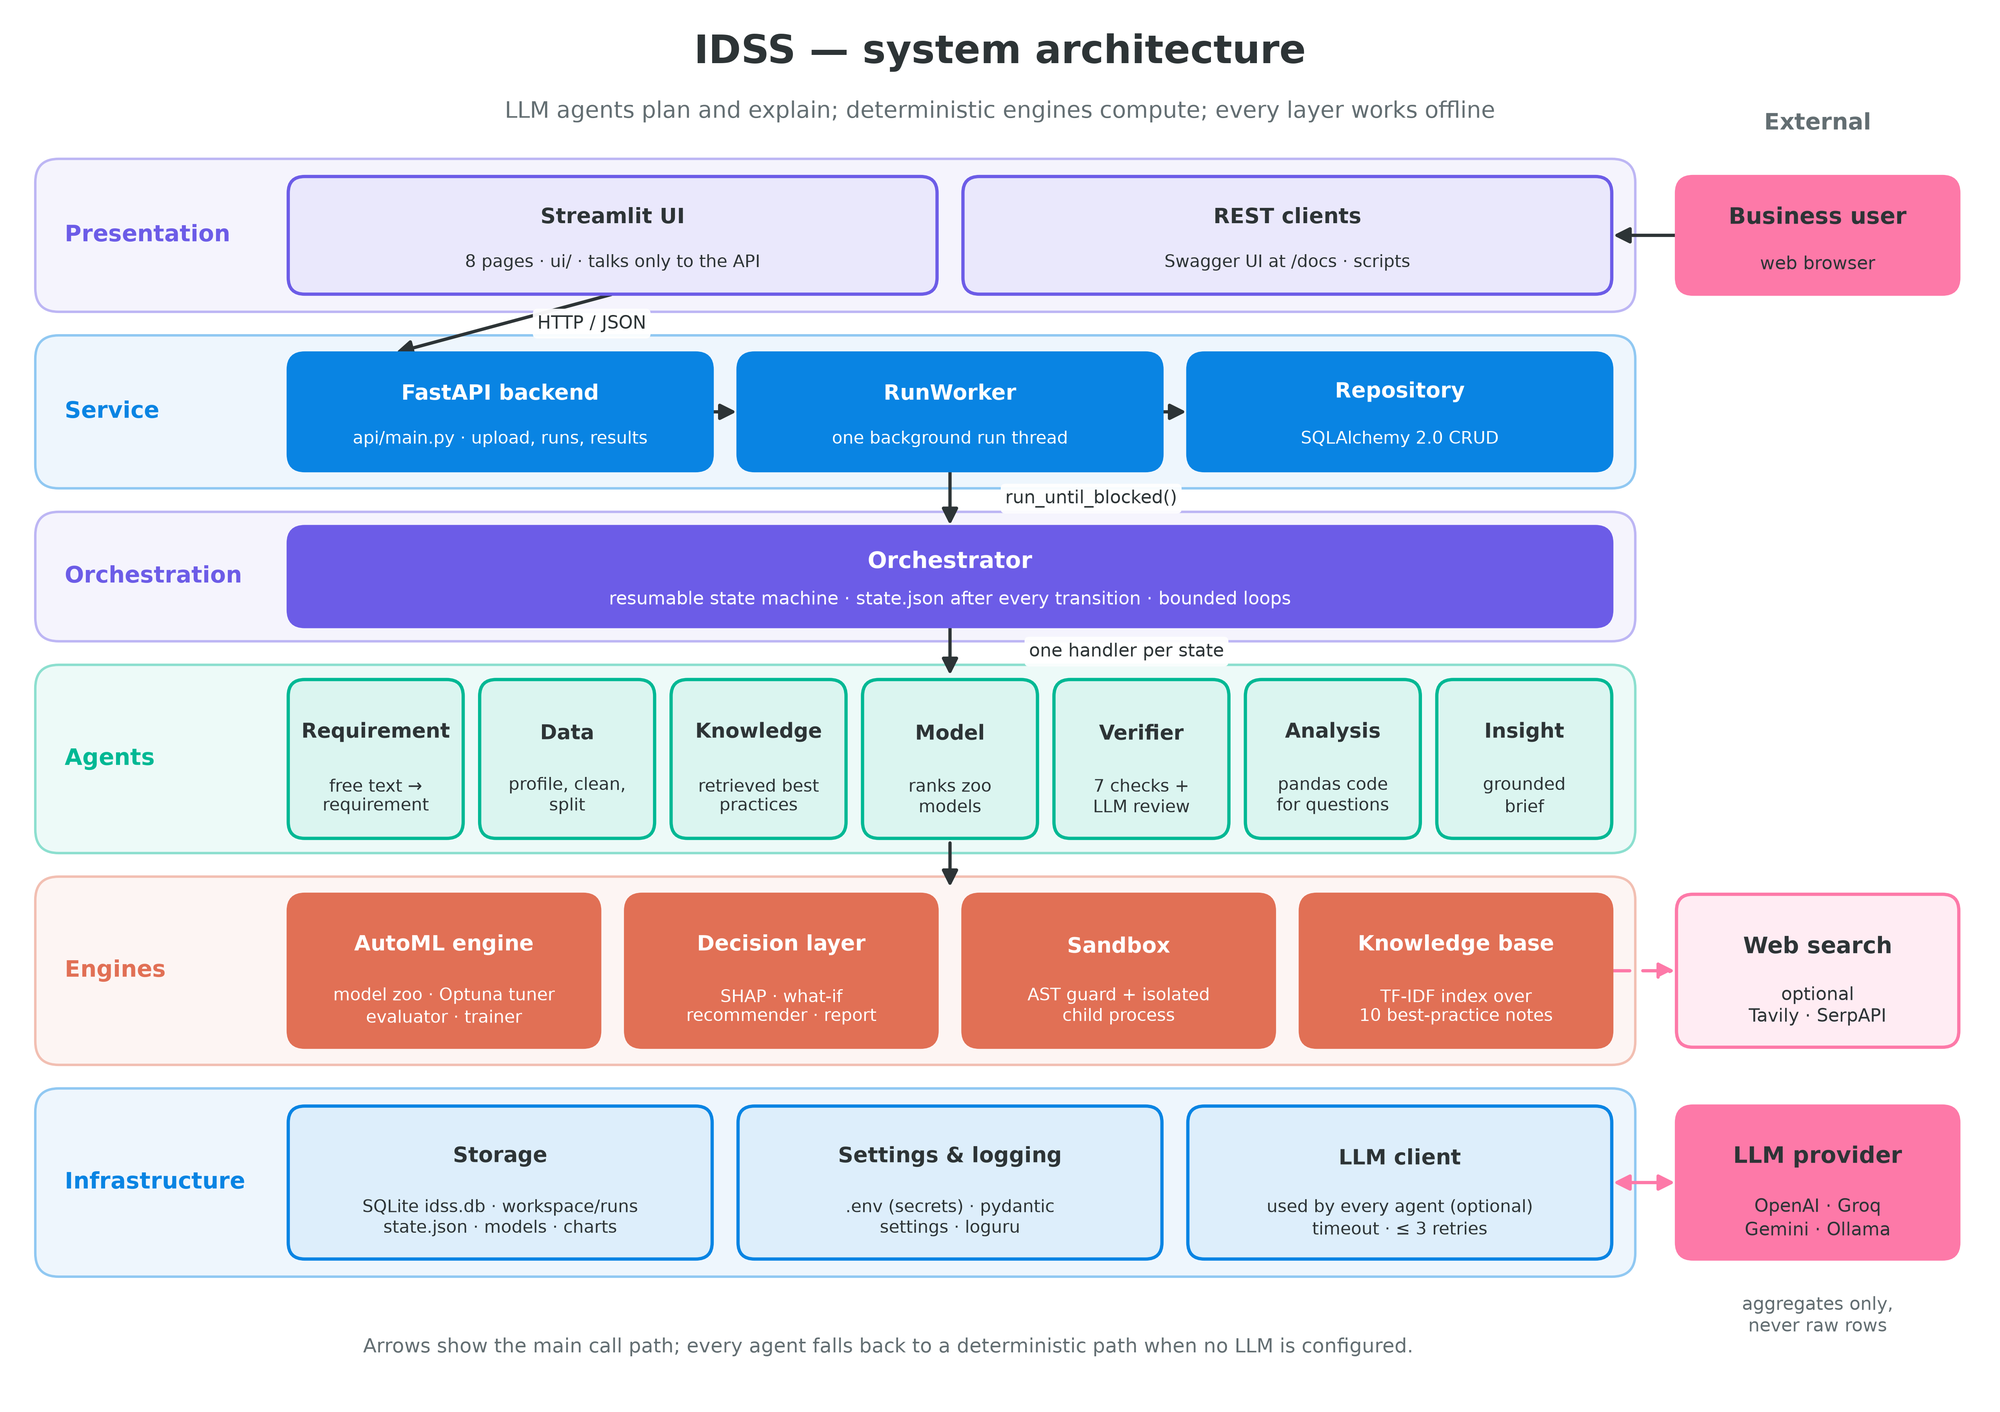
\includegraphics[width=\linewidth,height=7.3in,keepaspectratio]{figures/system_architecture.png}
  \caption{System architecture of IDSS}\label{fig:4.1}
\end{figure}

\begin{table}[H]
\centering
\linespread{1}\small
\setlength{\tabcolsep}{4pt}
\caption{Architectural layers}\label{tab:4.6}
\begin{tabular}{|>{\raggedright\arraybackslash\hspace{0pt}}p{\dimexpr 0.2231\linewidth-2\tabcolsep-2\arrayrulewidth\relax}|>{\raggedright\arraybackslash\hspace{0pt}}p{\dimexpr 0.3897\linewidth-2\tabcolsep-2\arrayrulewidth\relax}|>{\raggedright\arraybackslash\hspace{0pt}}p{\dimexpr 0.3872\linewidth-2\tabcolsep-2\arrayrulewidth\relax}|}
\hline
\rowcolor{tableheader}\textbf{Layer} & \textbf{Components} & \textbf{Code} \\
\hline
Presentation & Streamlit UI (8 pages), talks only to the API & \code{ui/} \\ \hline
Service & FastAPI backend, RunWorker thread, repository & \code{api/}, \code{idss/\allowbreak{}storage/} \\ \hline
Orchestration & Resumable state machine, one handler per state & \code{idss/\allowbreak{}agents/\allowbreak{}manager.\allowbreak{}py} \\ \hline
Agents & Requirement, Data, Knowledge, Model, Verifier, Analysis, Insight & \code{idss/\allowbreak{}agents/} \\ \hline
Engines & AutoML engine, decision layer, knowledge base, sandbox & \code{idss/\allowbreak{}ml/}, \code{idss/\allowbreak{}decision/}, \code{idss/\allowbreak{}knowledge/}, \code{idss/\allowbreak{}execution/} \\ \hline
Infrastructure & LLM client, SQLite and run workspace, settings, logging & \code{idss/\allowbreak{}core/}, \code{idss/\allowbreak{}storage/}, \code{configs/} \\ \hline
\end{tabular}
\end{table}

\FloatBarrier
\section{Data Flow Diagrams}\label{sec:4.4}

\textbf{Level 0.} Figure~\ref{fig:4.2} shows IDSS as one process and its external entities. The business user sends a dataset, a question, answers and what-if changes, and receives the profile, progress, clarifying questions, results, actions and the report. The optional LLM provider receives prompts with aggregates only and returns structured JSON; the optional web search service receives queries and returns snippets. Without an LLM, these flows are skipped.

\begin{figure}[htbp]
  \centering
  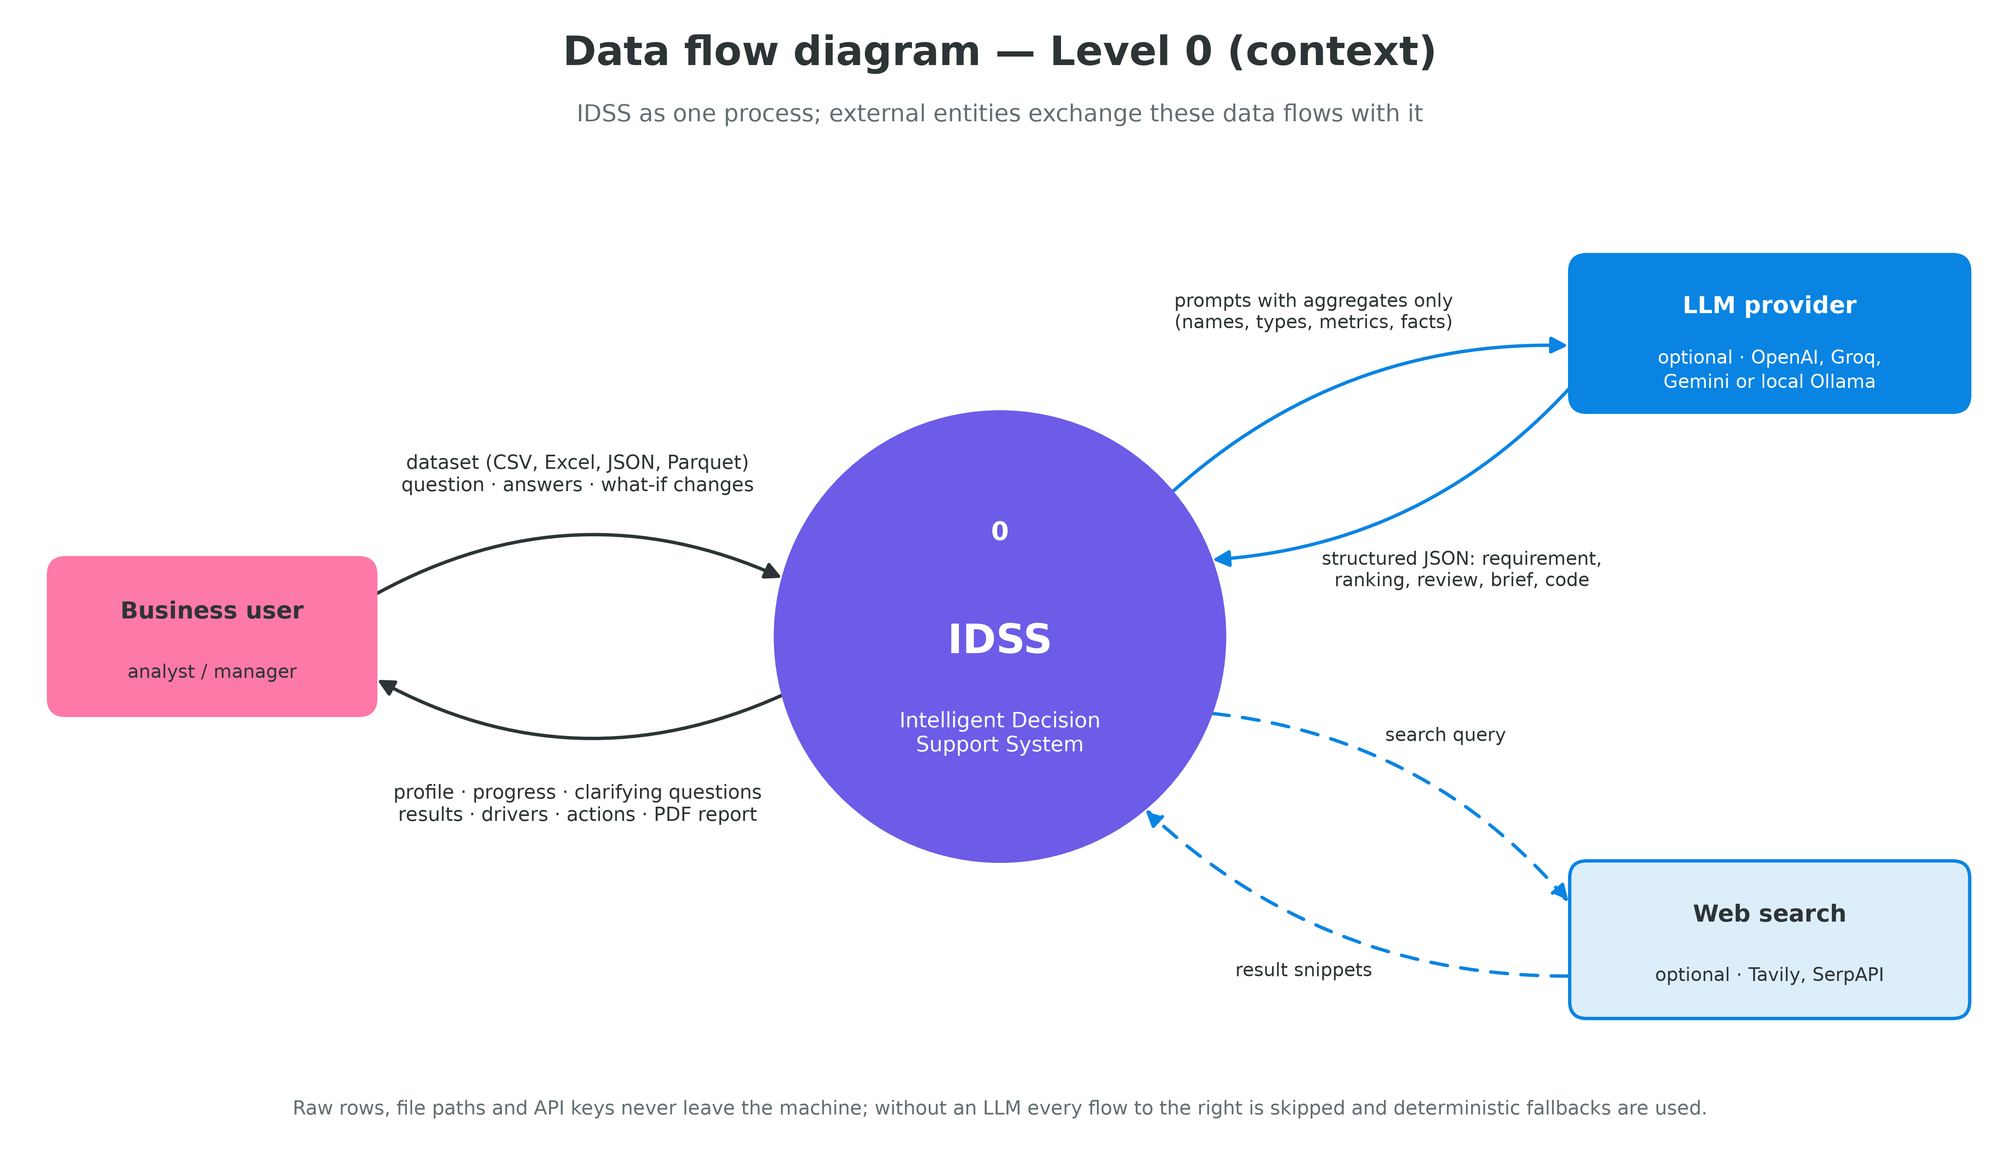
\includegraphics[width=\linewidth,height=7.3in,keepaspectratio]{figures/dfd_level0.png}
  \caption{Data flow diagram, Level 0 (context diagram)}\label{fig:4.2}
\end{figure}

\textbf{Level 1.} Figure~\ref{fig:4.3} decomposes the process. The file is loaded and profiled, cleaned, split 70/20/10 and preprocessed. Candidate models are tuned on the train and validation splits, the best compliant one is selected (with its decision threshold), refitted on train + validation and scored \textbf{once} on the held-out test split with a baseline, then verified and explained. Finally the system derives decisions, writes the grounded insight and builds the report. The run folder stores state, splits, model, charts and reports; SQLite indexes datasets, runs and events.

\begin{figure}[htbp]
  \centering
  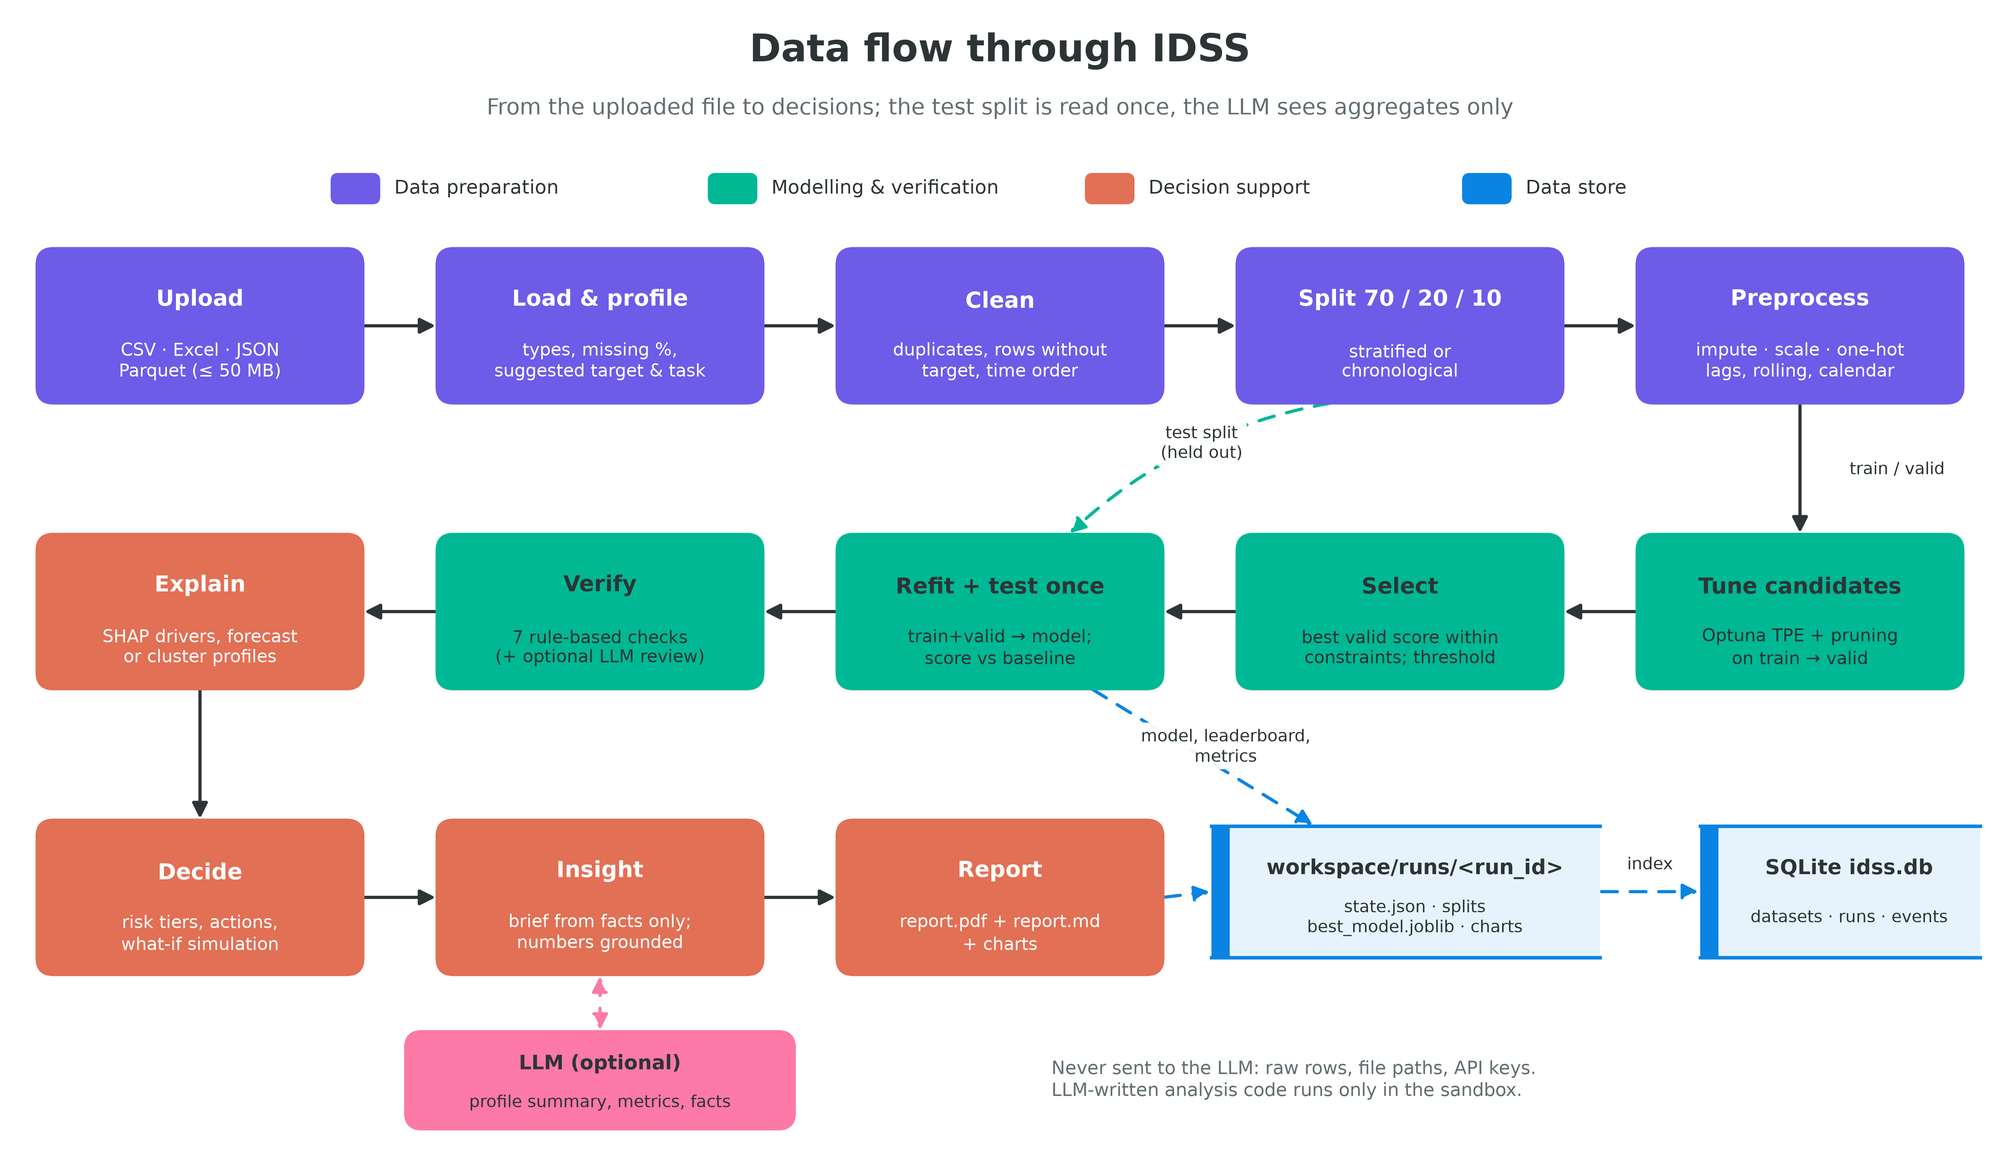
\includegraphics[width=\linewidth,height=7.3in,keepaspectratio]{figures/data_flow.png}
  \caption{Data flow diagram, Level 1}\label{fig:4.3}
\end{figure}

\FloatBarrier
\section{UML Diagrams}\label{sec:4.5}

\subsection{Use Case Diagram}\label{sec:4.5.1}

The business user uploads and profiles data, describes the problem (extended by answering clarifying questions), monitors runs, views results and verification, explores drivers, reviews recommendations and risk tiers, simulates what-if scenarios, asks questions about the data and downloads reports. A team member runs the evaluation and the tests and regenerates samples and diagrams. The LLM provider is an optional external system (Figure~\ref{fig:4.4}).

\begin{figure}[htbp]
  \centering
  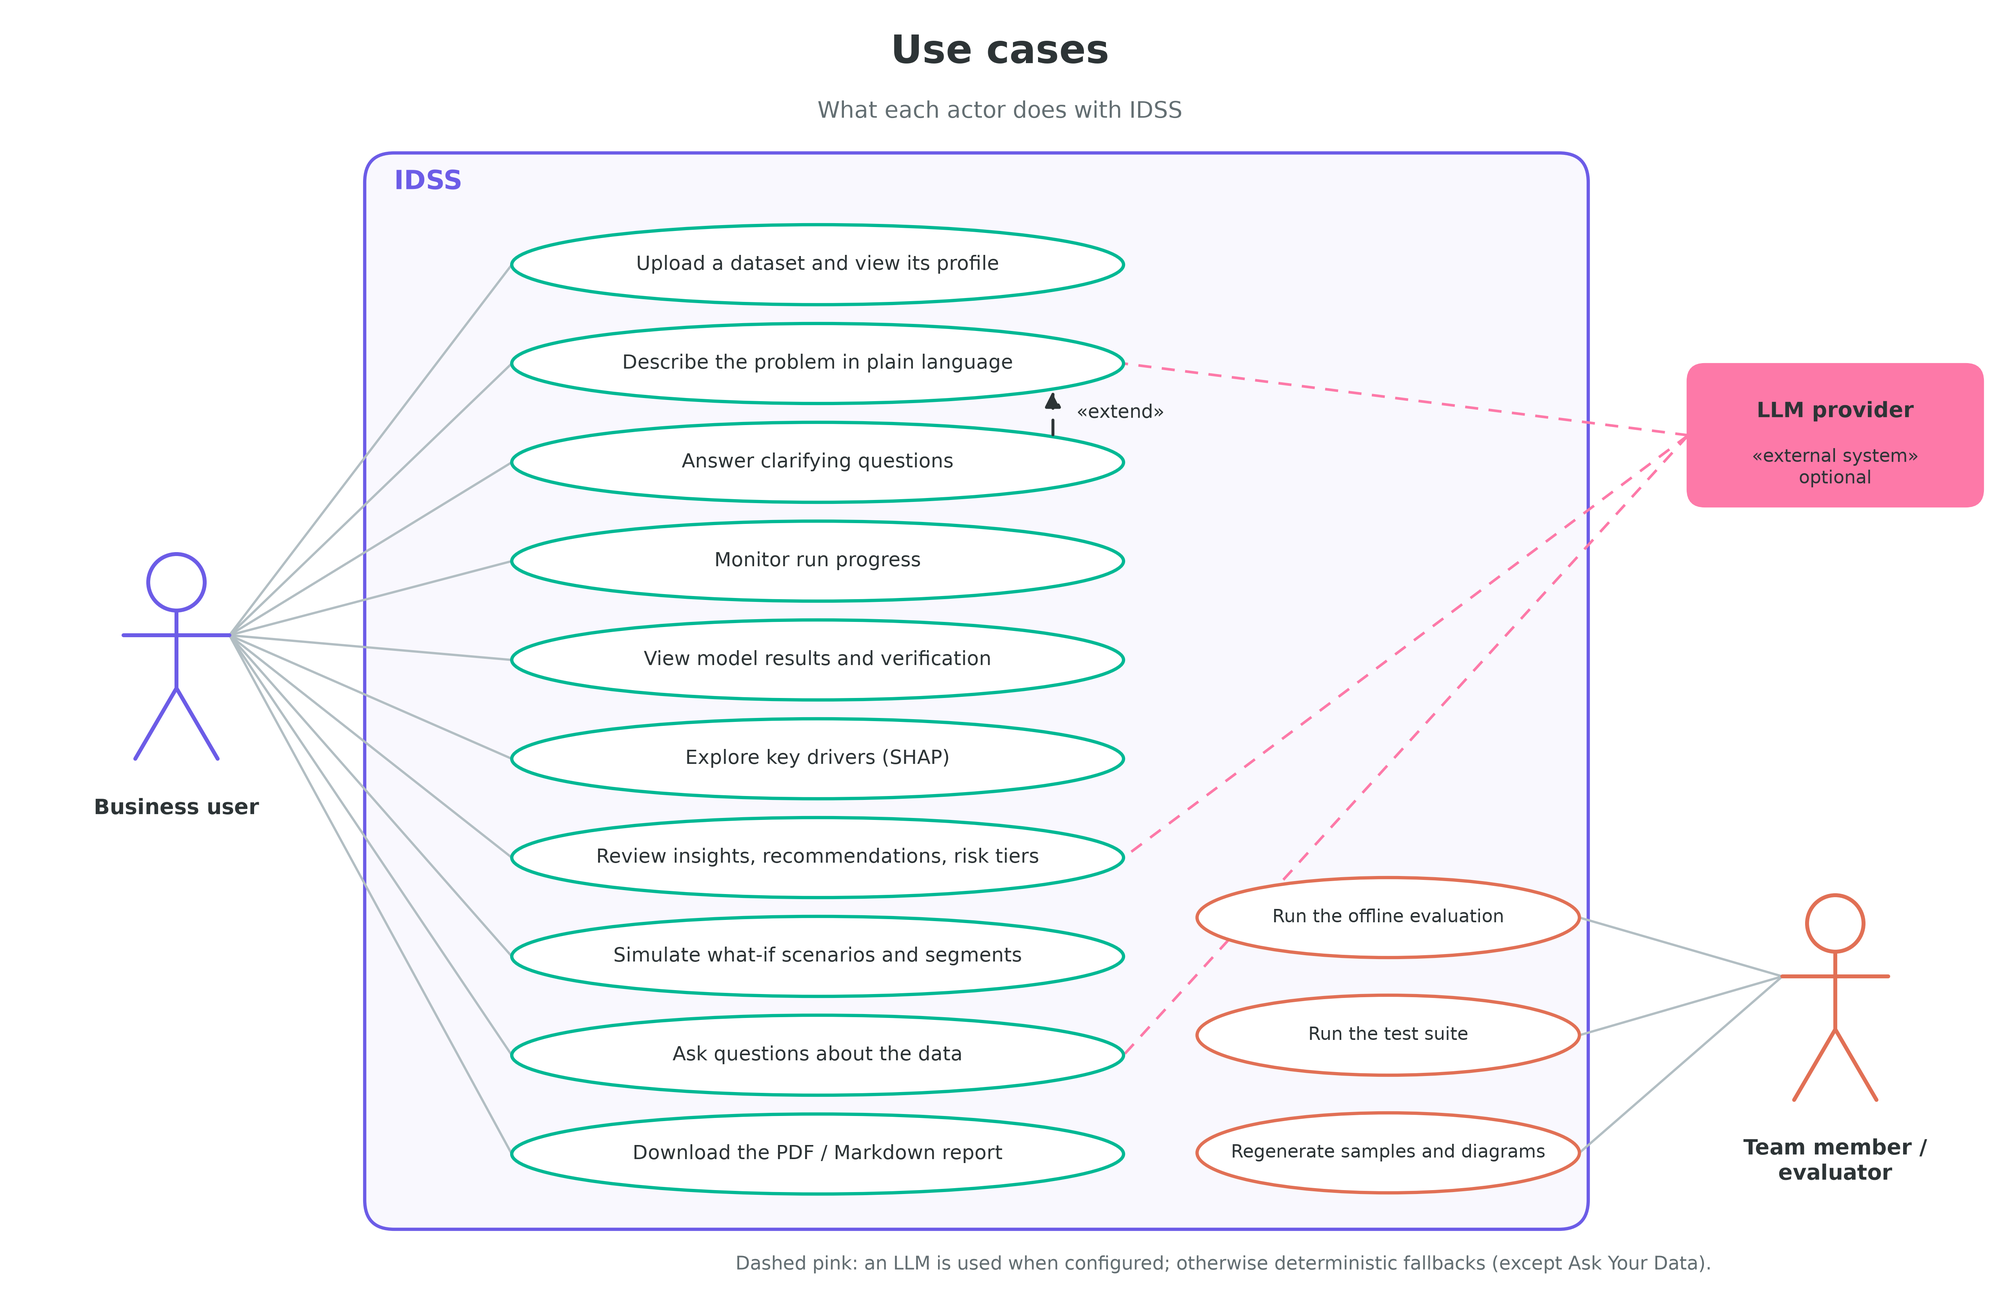
\includegraphics[width=\linewidth,height=7.3in,keepaspectratio]{figures/use_case.png}
  \caption{Use case diagram}\label{fig:4.4}
\end{figure}

\subsection{Class Diagram}\label{sec:4.5.2}

The \textbf{Orchestrator} owns one instance of each agent and the current \textbf{RunContext}, which holds the whole state of a run and is saved as \code{state.json}; it mirrors every transition into the \textbf{Repository} and is driven by the API's \textbf{RunWorker}. Every agent holds an optional \textbf{LLMClient}. The \textbf{KnowledgeAgent} queries the \textbf{KnowledgeIndex}; in the TRAIN state the \textbf{AutoMLTrainer} creates a \textbf{TrainedModel} and reads the test split through the \textbf{Holdout}, whose access log proves a single read; the \textbf{ModelExplainer} explains a TrainedModel (Figure~\ref{fig:4.5}).

\begin{figure}[htbp]
  \centering
  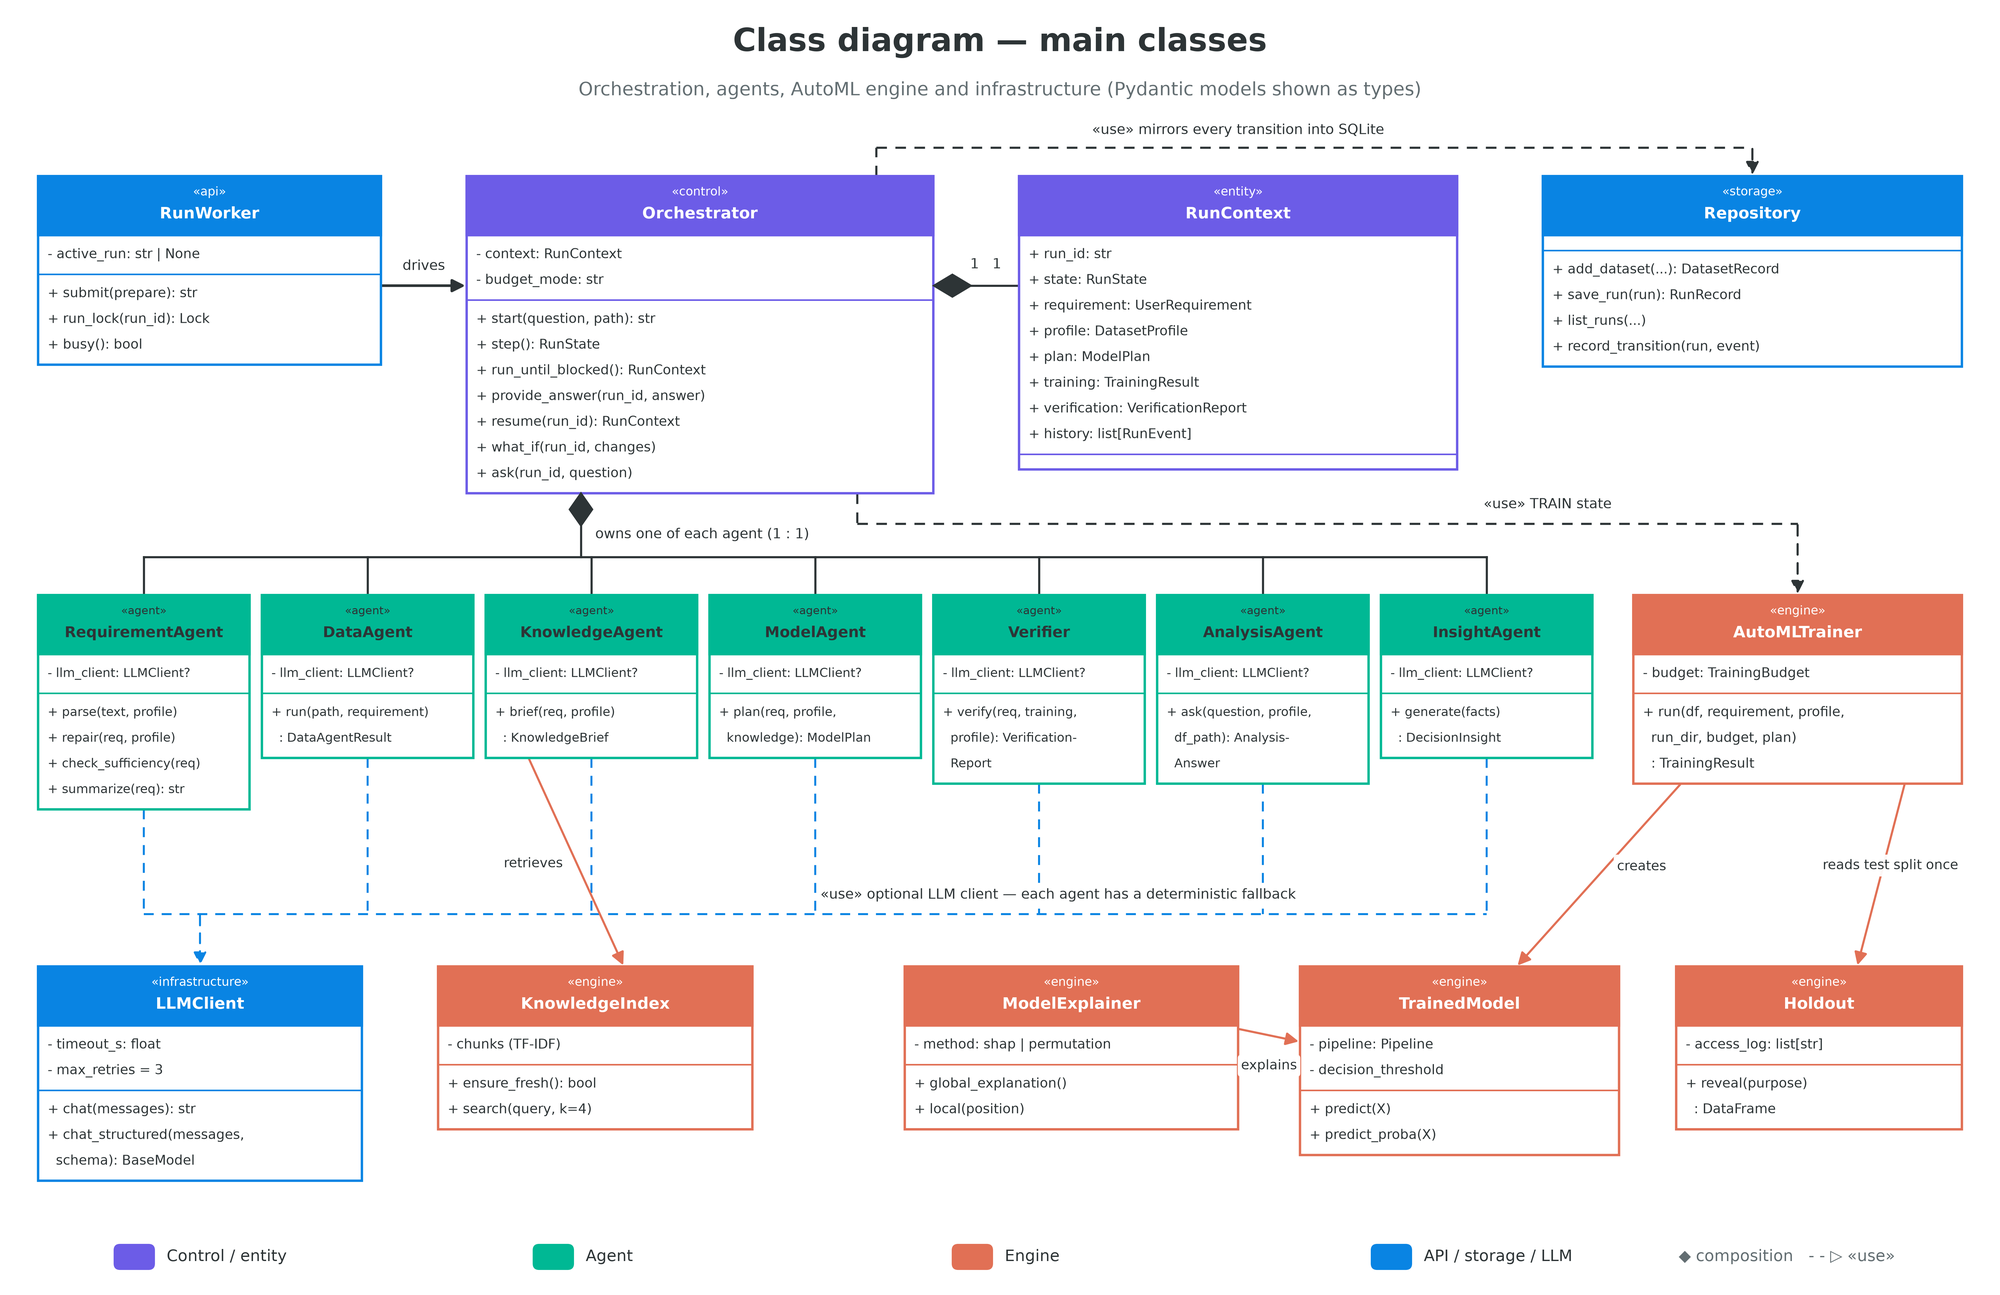
\includegraphics[width=\linewidth,height=7.3in,keepaspectratio]{figures/class_diagram.png}
  \caption{Class diagram of the main classes}\label{fig:4.5}
\end{figure}

\subsection{Sequence Diagram}\label{sec:4.5.3}

The user uploads a CSV; the API saves it, caches its profile and returns the dataset id. The user starts an analysis; the API hands the run to the RunWorker and returns \code{202} at once. The Orchestrator runs the agents, the AutoML engine and the decision steps, saving \code{state.json} and an event after every transition, while the UI polls \code{GET /\allowbreak{}runs/\allowbreak{}\{id\}} every two seconds. Finally the user opens results and reports and runs a what-if with the trained model (Figure~\ref{fig:4.6}).

\begin{figure}[htbp]
  \centering
  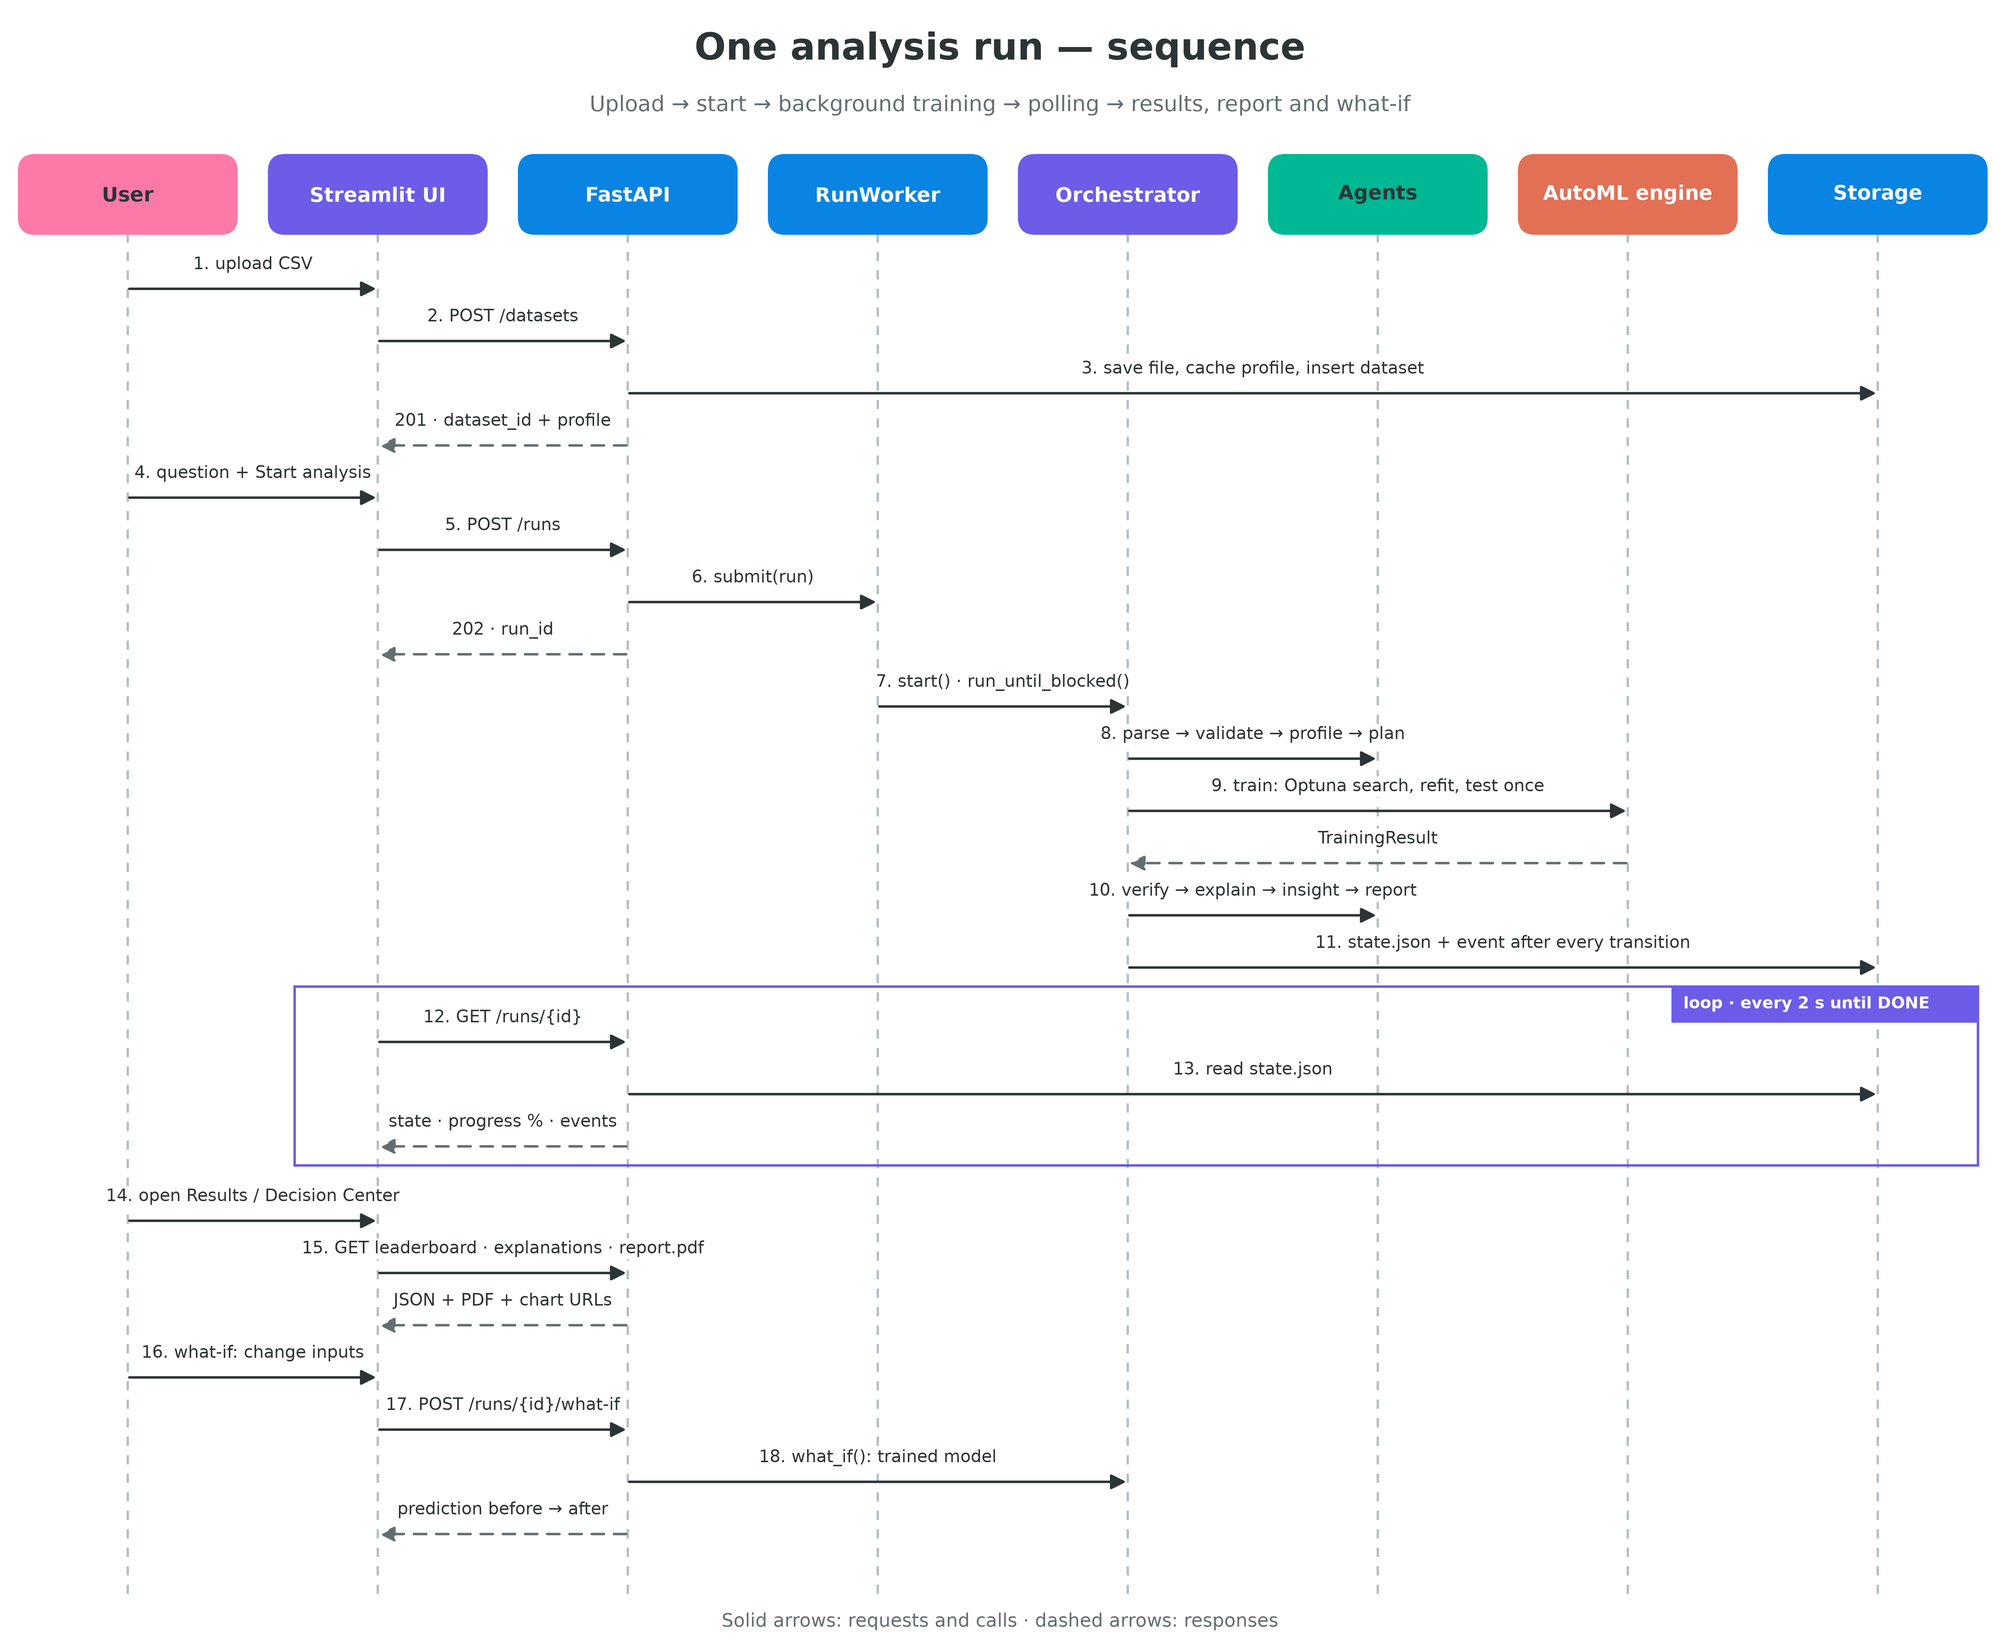
\includegraphics[width=\linewidth,height=7.3in,keepaspectratio]{figures/sequence_one_run.png}
  \caption{Sequence diagram of one analysis run}\label{fig:4.6}
\end{figure}

\subsection{State Chart Diagram}\label{sec:4.5.4}

Each state has one handler that returns the next state. INIT checks relevance (an irrelevant request ends in DONE with a polite reply); PARSE and VALIDATE build and check the requirement, waiting in NEEDS\_INPUT for answers (at most two rounds); PROFILE, PLAN, TRAIN and VERIFY build and check the model; a failed check returns once to PLAN with the full budget, after which the run continues flagged \textit{not verified}; EXPLAIN, INSIGHT and REPORT produce the decision support. Any unhandled error moves the run to FAILED (Figure~\ref{fig:4.7}).

\begin{figure}[htbp]
  \centering
  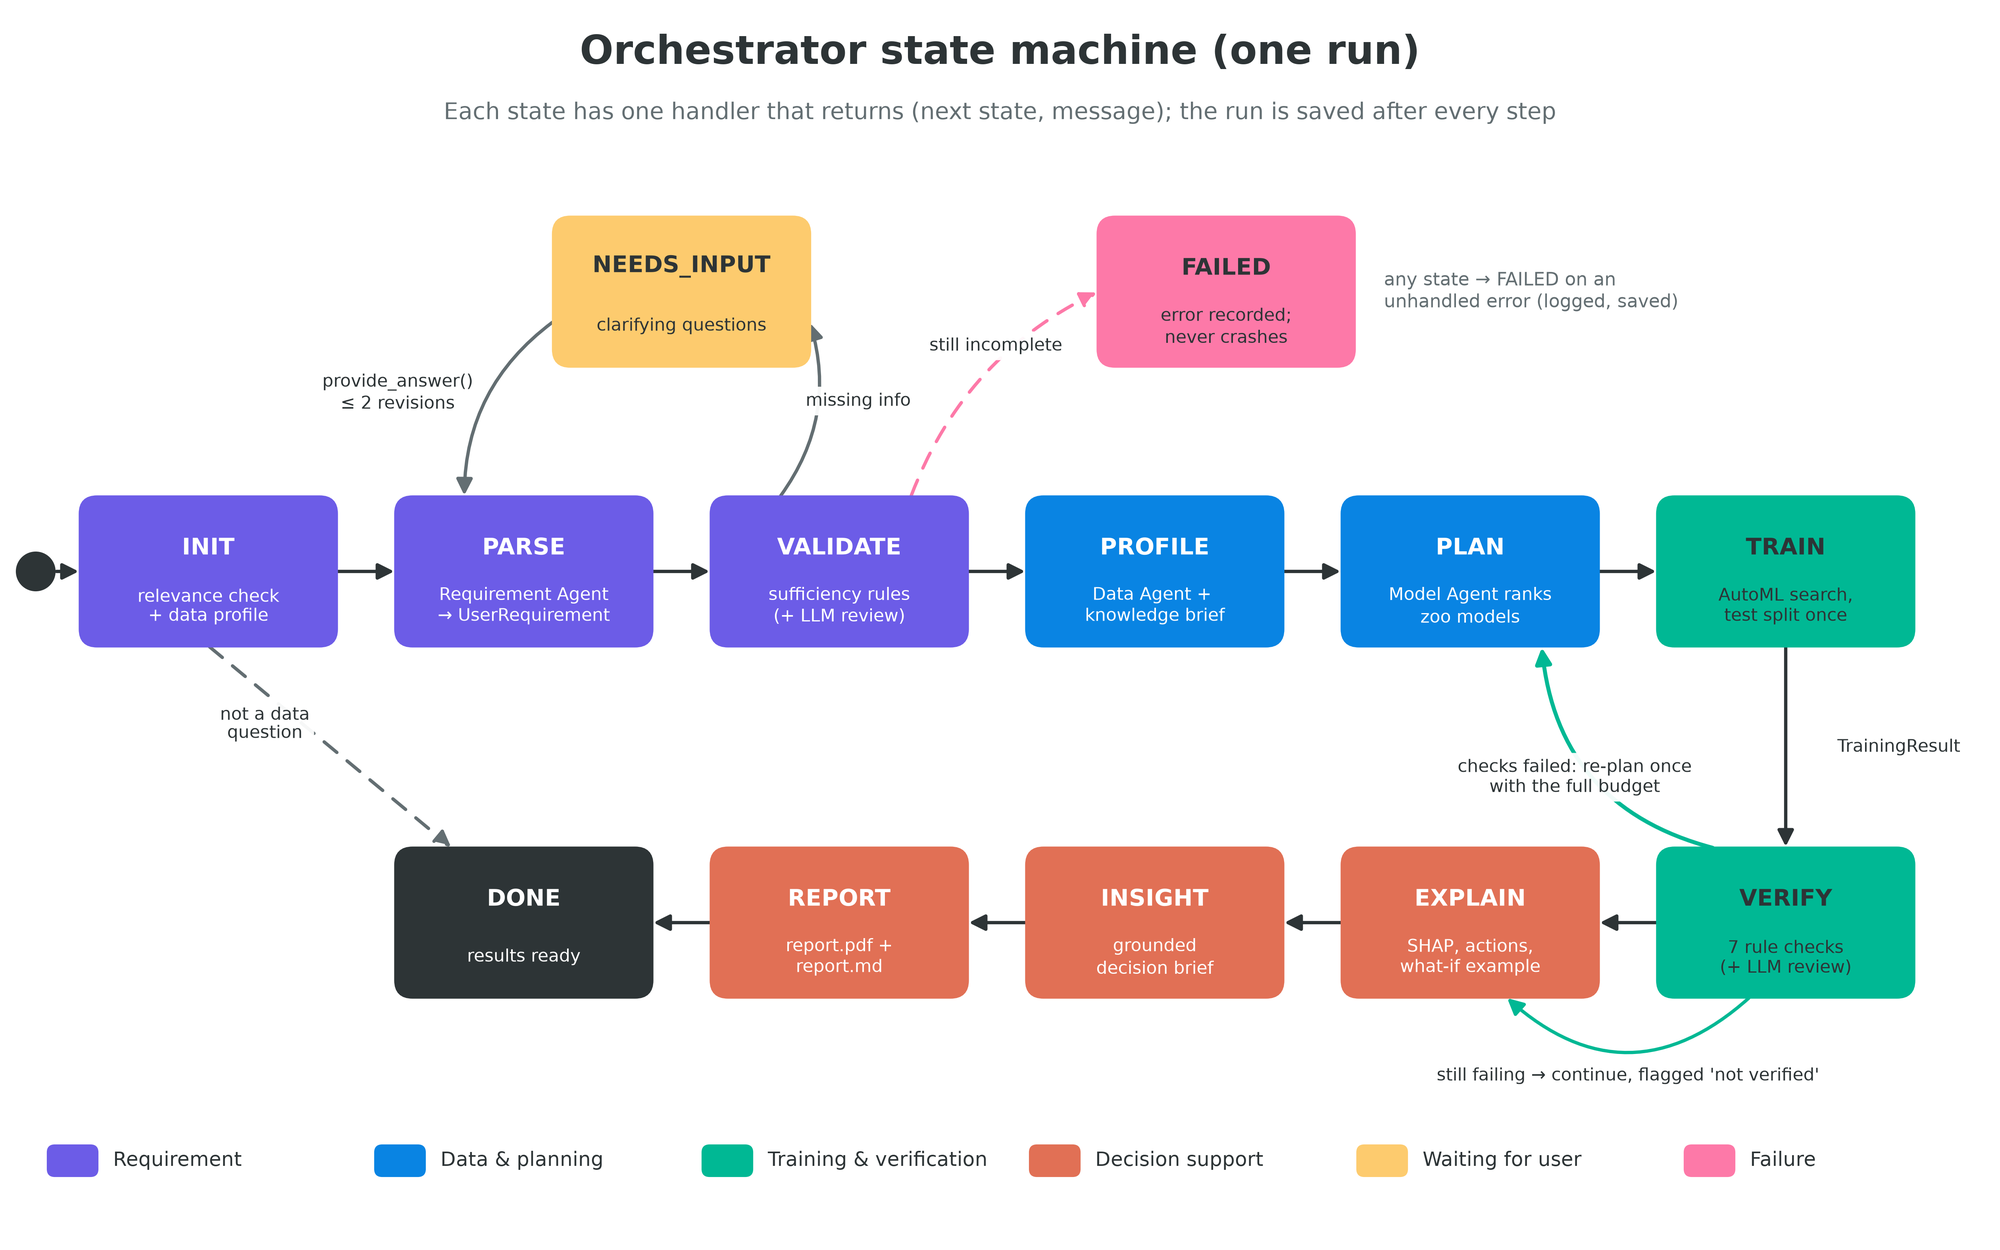
\includegraphics[width=\linewidth,height=7.3in,keepaspectratio]{figures/agent_workflow.png}
  \caption{State chart diagram of a run}\label{fig:4.7}
\end{figure}

\subsection{Activity Diagram}\label{sec:4.5.5}

Figure~\ref{fig:4.8} shows one analysis in four swimlanes --- business user, UI and API, Orchestrator and agents, engines --- with the three decision points of the workflow: is the request relevant, is enough information available, and did verification pass.

\begin{figure}[htbp]
  \centering
  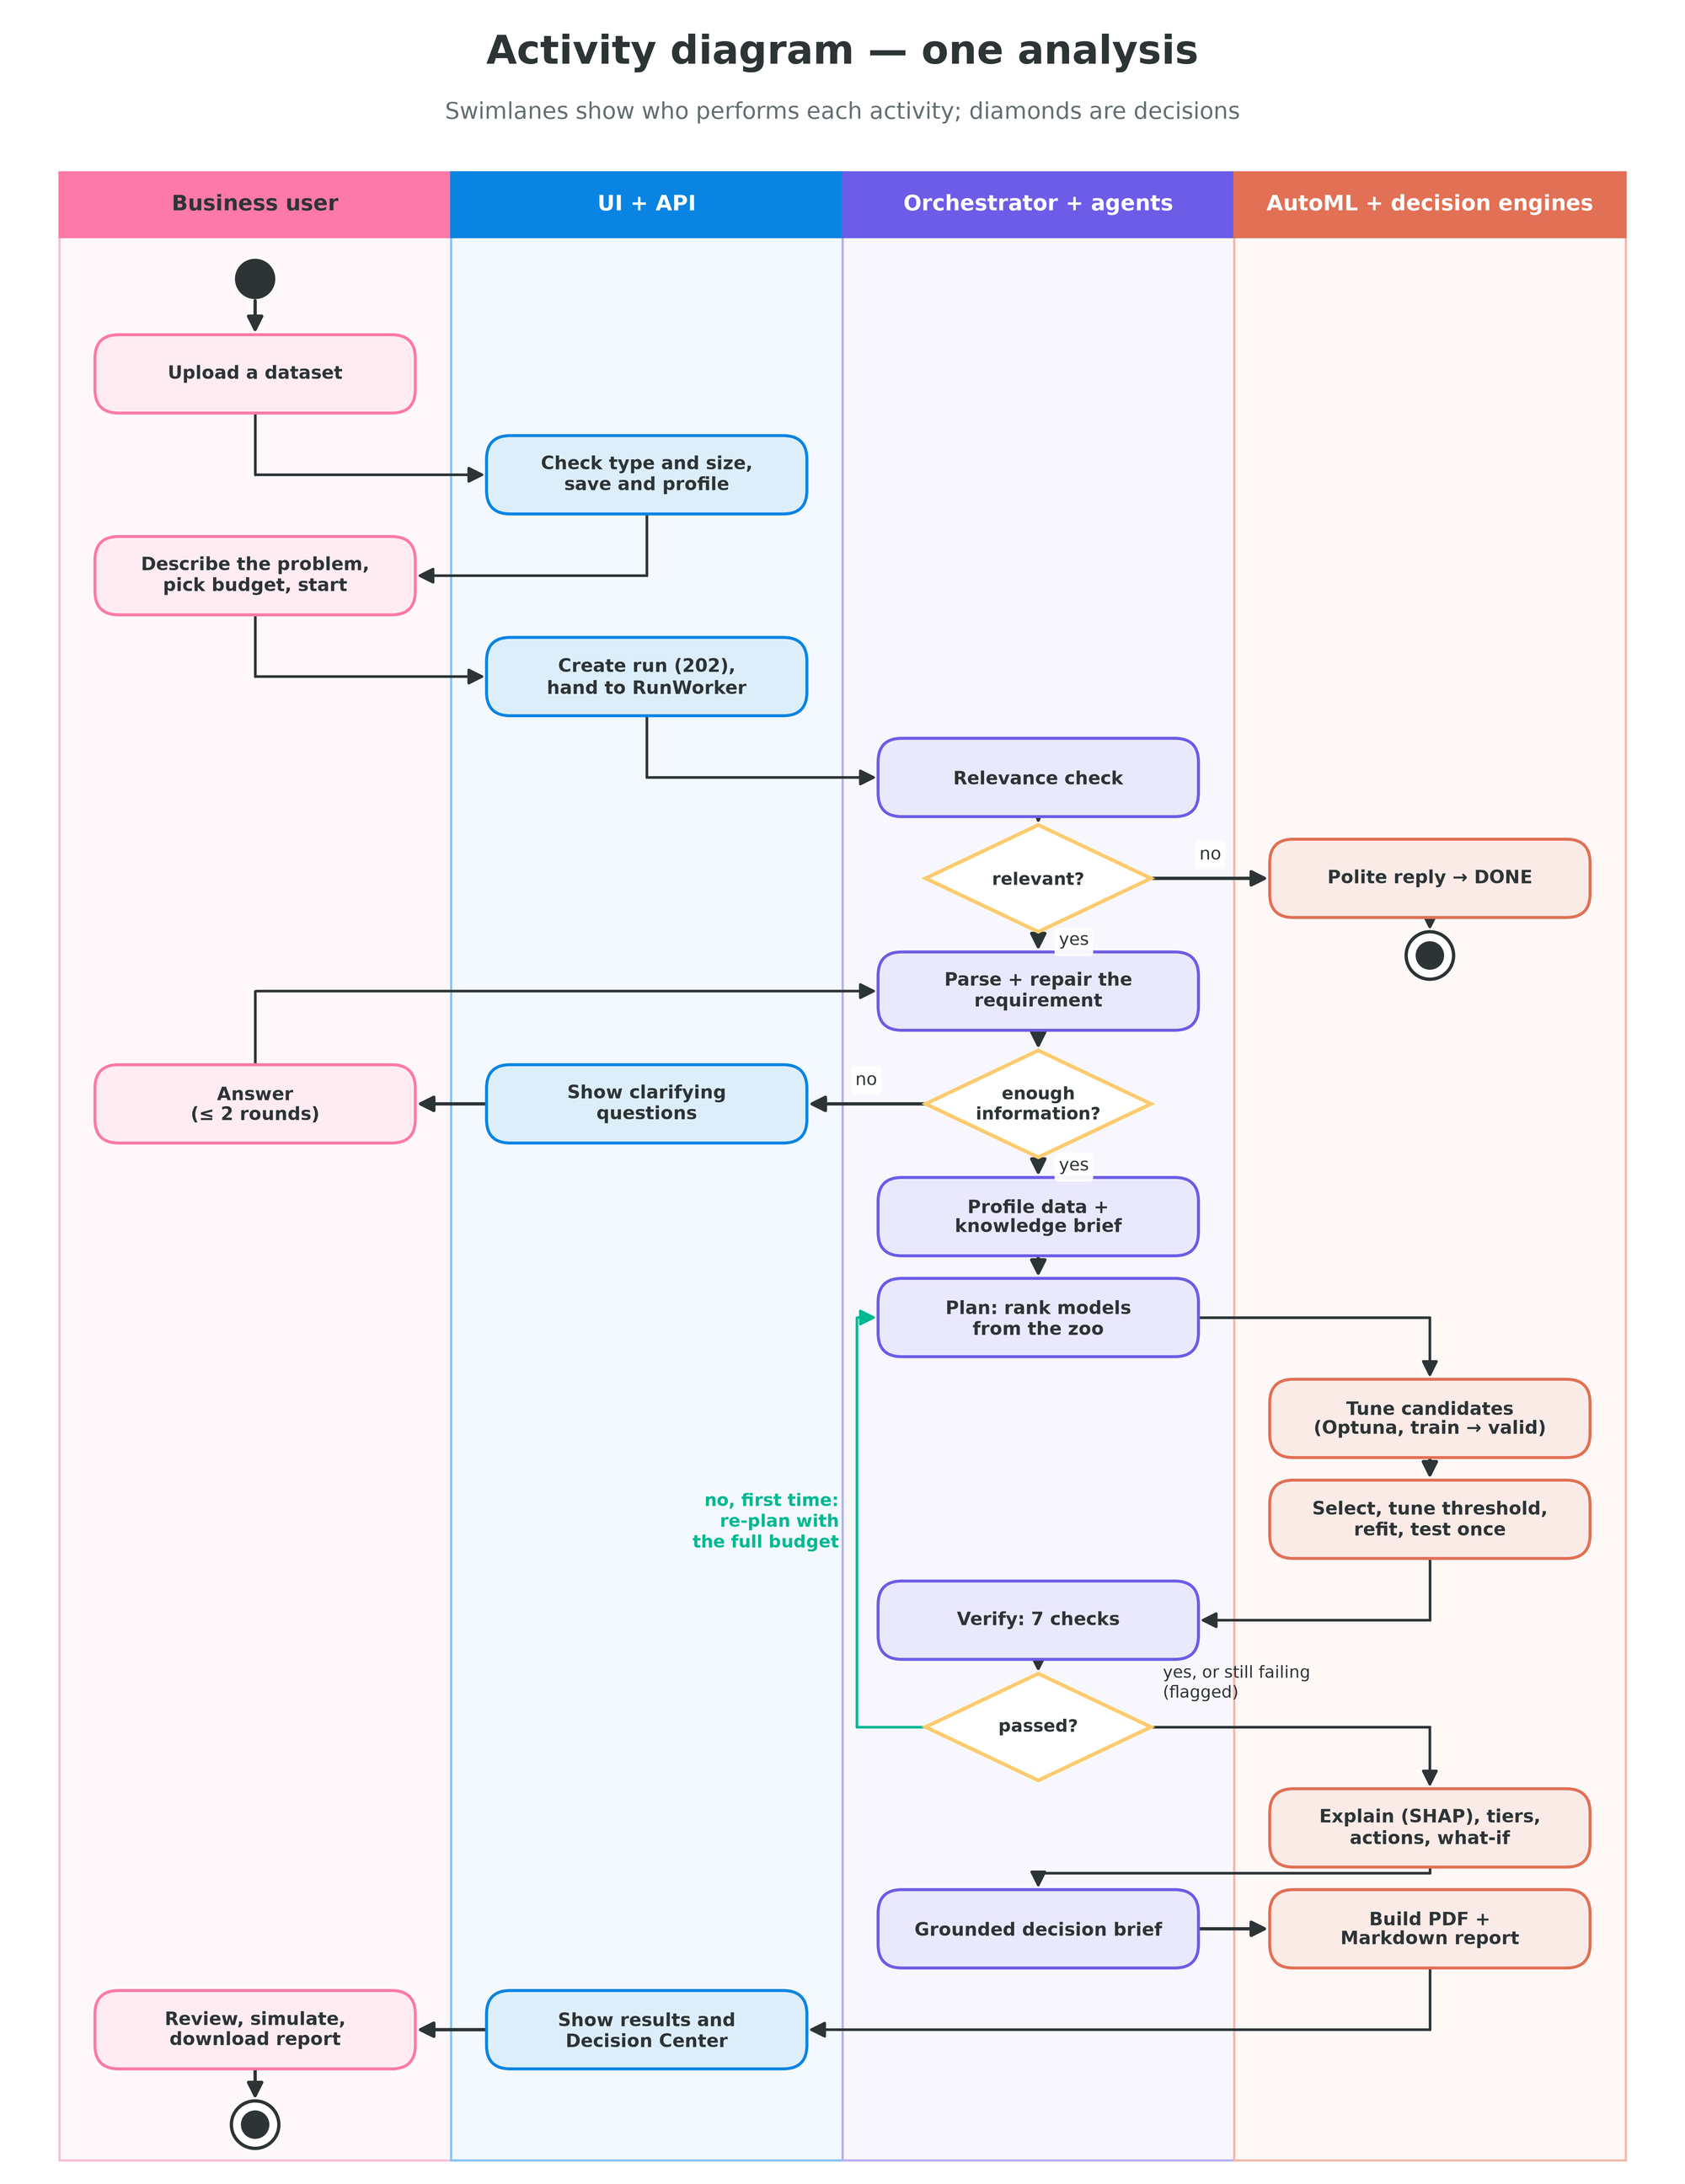
\includegraphics[width=\linewidth,height=7.3in,keepaspectratio]{figures/activity_diagram.png}
  \caption{Activity diagram of one analysis}\label{fig:4.8}
\end{figure}

\subsection{Component and Deployment Diagram}\label{sec:4.5.6}

Everything runs on one Windows PC. The browser shows the dashboard served by the Streamlit process (port 8501), whose pages call the Uvicorn + FastAPI process (port 8000) over \code{127.0.0.1}. Inside the API process, the routes hand work to the RunWorker thread (Orchestrator, agents, engines) and the storage component reads and writes \code{workspace/}. \textit{Ask Your Data} spawns a separate sandbox process. The LLM provider and web search are optional external services, and \code{.env} is read only by the API process (Figure~\ref{fig:4.9}).

\begin{figure}[htbp]
  \centering
  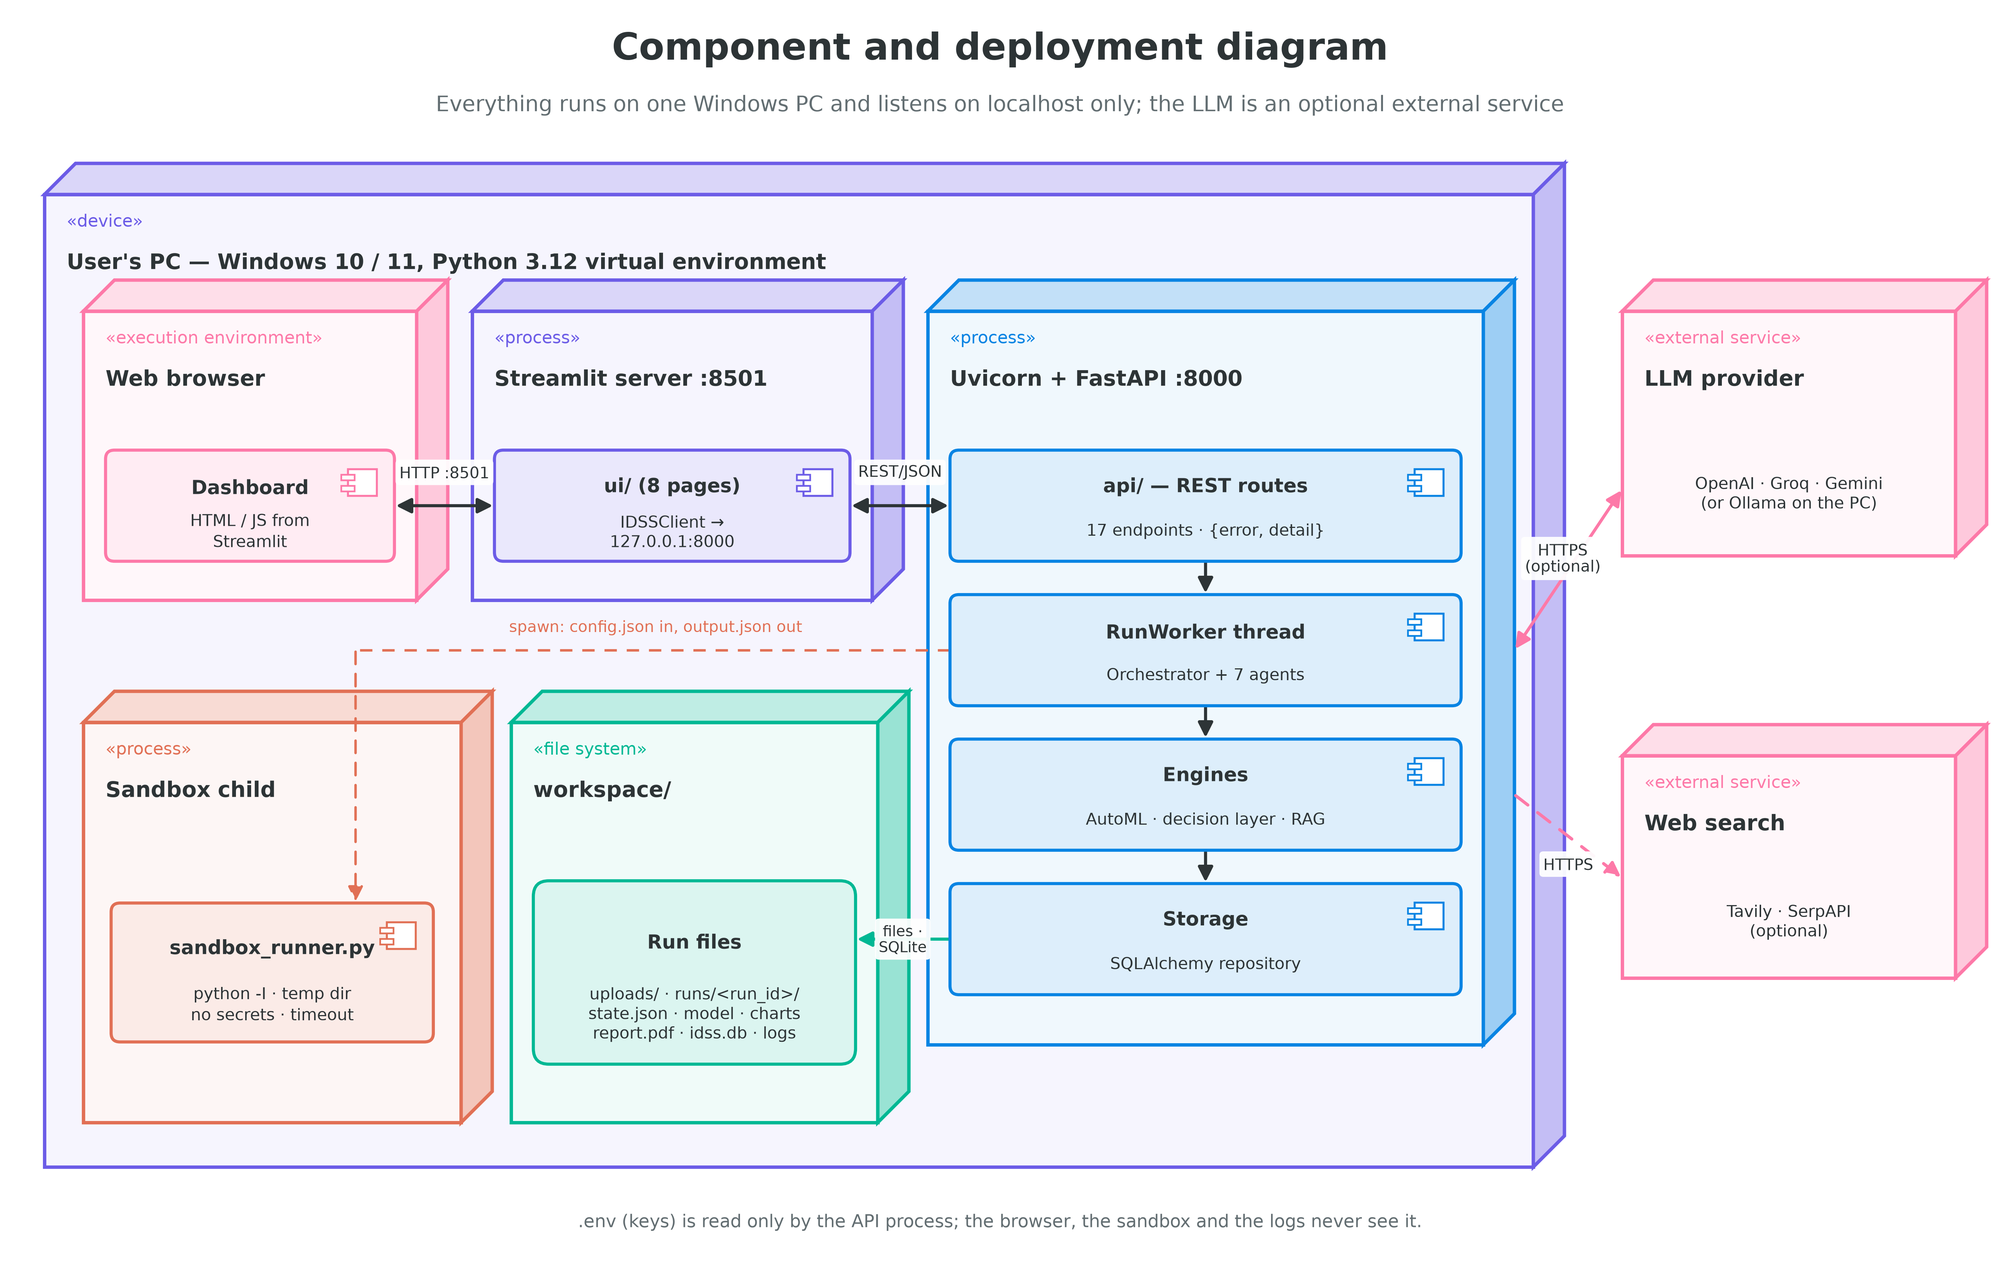
\includegraphics[width=\linewidth,height=7.3in,keepaspectratio]{figures/deployment_diagram.png}
  \caption{Component and deployment diagram}\label{fig:4.9}
\end{figure}

\FloatBarrier
\section{Database Design}\label{sec:4.6}

Each run's \code{state.json} is the source of truth; an SQLite database (\code{workspace/\allowbreak{}idss.db}, write-ahead logging, foreign keys on) indexes datasets, runs and events for fast listing (Figure~\ref{fig:4.10}, Table~\ref{tab:4.7}). A dataset is used by many runs (on delete: set null) and a run has many events (on delete: cascade). The Orchestrator writes the run and its newest event in one transaction after every transition; a database error is only logged.

\begin{figure}[htbp]
  \centering
  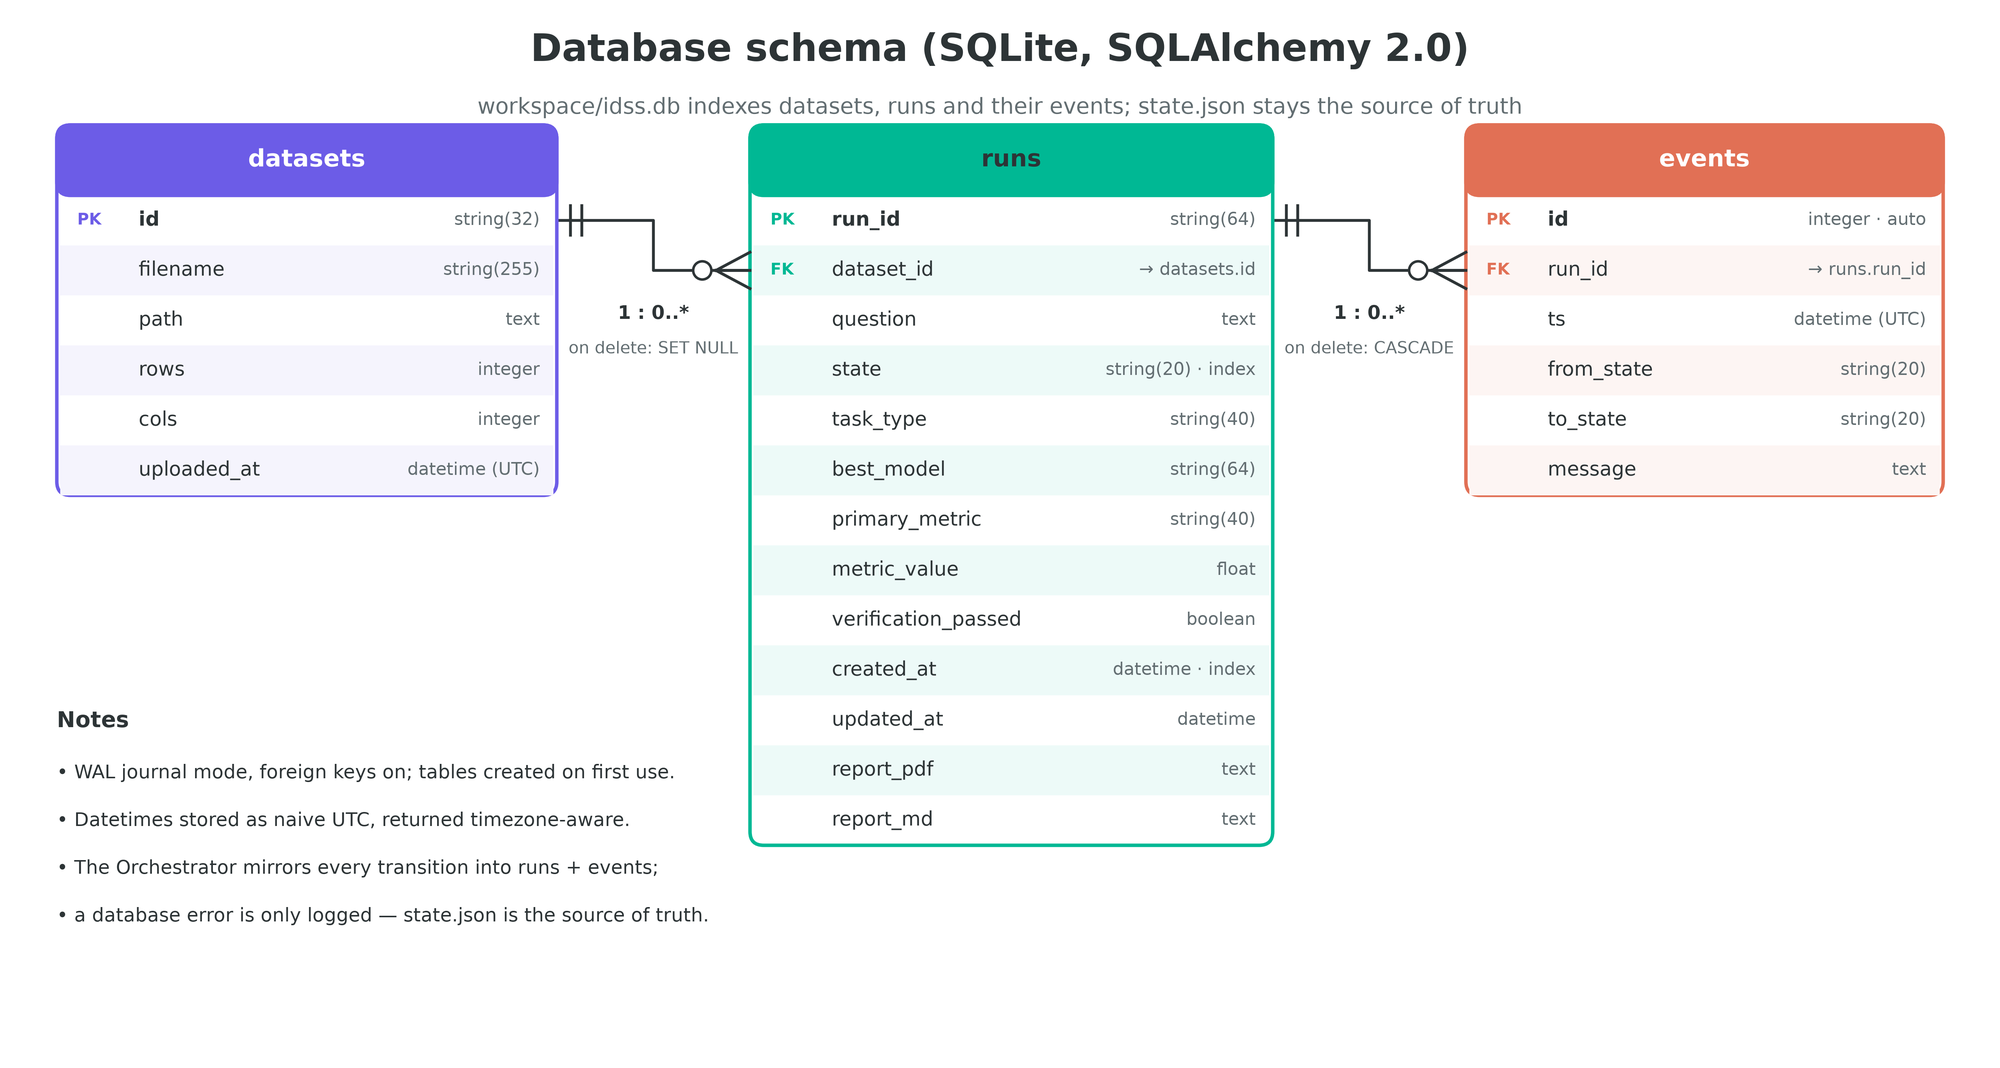
\includegraphics[width=\linewidth,height=7.3in,keepaspectratio]{figures/er_diagram.png}
  \caption{Entity--relationship diagram of the database}\label{fig:4.10}
\end{figure}

\begin{table}[H]
\centering
\linespread{1}\small
\setlength{\tabcolsep}{4pt}
\caption{Database tables}\label{tab:4.7}
\begin{tabular}{|>{\raggedright\arraybackslash\hspace{0pt}}p{\dimexpr 0.1414\linewidth-2\tabcolsep-2\arrayrulewidth\relax}|>{\raggedright\arraybackslash\hspace{0pt}}p{\dimexpr 0.5764\linewidth-2\tabcolsep-2\arrayrulewidth\relax}|>{\raggedright\arraybackslash\hspace{0pt}}p{\dimexpr 0.2821\linewidth-2\tabcolsep-2\arrayrulewidth\relax}|}
\hline
\rowcolor{tableheader}\textbf{Table} & \textbf{Key columns} & \textbf{Purpose} \\
\hline
\code{datasets} & \code{id} (PK), \code{filename}, \code{path}, \code{rows}, \code{cols}, \code{uploaded\_\allowbreak{}at} & One row per uploaded file \\ \hline
\code{runs} & \code{run\_\allowbreak{}id} (PK), \code{dataset\_\allowbreak{}id} (FK), \code{question}, \code{state}, \code{task\_\allowbreak{}type}, \code{best\_\allowbreak{}model}, \code{primary\_\allowbreak{}metric}, \code{metric\_\allowbreak{}value}, \code{verification\_\allowbreak{}passed}, timestamps, report paths & Summary of each run \\ \hline
\code{events} & \code{id} (PK), \code{run\_\allowbreak{}id} (FK), \code{ts}, \code{from\_\allowbreak{}state}, \code{to\_\allowbreak{}state}, \code{message} & One row per state transition \\ \hline
\end{tabular}
\end{table}

\FloatBarrier
\section{Summary}\label{sec:4.7}

This chapter specified twenty functional and thirteen non-functional requirements, the data, hardware and software requirements and an SRS summary, and presented the design: a six-layer architecture, Level 0 and Level 1 data flow diagrams, six UML views and the database schema.
